\documentclass[10pt,]{article}

\usepackage{xspace}
\usepackage{amsmath,amssymb}
\usepackage{adjustbox}
\usepackage[dvipsnames]{xcolor}
\usepackage{multirow}
\usepackage{datetime}
\usepackage{caption}
\usepackage{subcaption}
\usepackage{hyperref}
\usepackage[toc,page]{appendix}
\usepackage[normalem]{ulem} % strikethrough

%% Use these lines for letter-sized paper
\usepackage[paper=letterpaper,
%%             nofoot, % Uncomment to put page number above margin
%%             marginparwidth=1in,     % Length of section titles
%%             marginparsep=.05in,       % Space between titles and text
               margin=1in,               % 1 inch margins
            left=0.75in,
            right=0.75in,
%%             includemp
            ]{geometry}

\title{The Endcap Thermal Model}
\date{\today, \currenttime}
\author{Kurt Brendlinger, Yu-Heng Chen, Sergio Diez Cornell, Claire David}

%% More layout: Get rid of indenting throughout entire document
\setlength{\parindent}{0in}
\setlength{\parskip}{2mm}

\begin{document}
\thispagestyle{empty}

%% \today, \currenttime

\maketitle

\tableofcontents

\section{Changes since the previous results}

{ \bf
December 12, 2018: The following adjustments were made to results since the version immediately
following ITK Week in November 2017:}
\begin{itemize}
\item The total analog current of the ABC is now set to 70 mA, based on the advice of Paul Keener.
(The ABC digital current is 42.5 mA.)
\item The ASIC-to-hybrid glue was updated to the ``UV cure glue'' described in the TDR. The previous
  glue used was tra-duct-2902.
\item The thermal conductivity of the PCB (powerboard) underneath the FEAST was changed from 0.3 to
3 Wm$^{-1}$K$^{-1}$, based on measurements and advice from Graham Beck. The barrel and endcap FEAST
thermal impedance values calculated from FEA are now more compatible. The result is a reduced FEAST
temperature in the model.
\item The model now includes two AMACs on R3 (powered by two LDOs); previously only one AMAC was used.
\item A 1.9 mA quiescent current is included in the LDOs providing power to the AMACs.
\end{itemize}

{\bf 
December 18, 2018: The following adjustments were made since circulation of the document on December 12, 2017:}
\begin{itemize}
\item The flux estimates have been changed from ``Step 1.9'' to the ``step 2.2 duals layout'' used in
the Pixel TDR. This should be the latest flux estimate.
\item A bug was fixed in which the pessimistic TID bump parameterization safety factor was not applied.
This increases the maximum power estimates slightly, in the worst-case scenario.
\end{itemize}

{ \bf
April 30, 2018: The following changes were made since December 18, 2018:}
% New system architecture: https://edms.cern.ch/ui/file/1807716/1.14/Full_System_Architecture_1.14_EDMS.pdf
\begin{itemize}
\item TODDO The FEAST is replaced by the BPOL12V, however the modeling of this converter (temperature
  and current dependence has not changed. The powering of the AMAC is now handled by the LINPOL12V
  instead of the BPOL12V (FEAST). This reduces the power associated to the FEAST, and thus the
  temperature.
\item The treatment of LV tape losses and FEAST voltages has now been made more consistent. Previously,
  tape resistances were modeled with a flat 10 m$\Omega$ resistance and FEAST voltages were set by hand.
  Now, the BPOL12V voltages are calculated on-the-fly using the voltage drop of the BPOL12V+tape of
  the previous modules. Currently the tape resistances are set by hand to force a 1V voltage decrease
  across the whole module. They should be updated with more realistic values. See Section~TODO.
\item Modules R3, R4 and R5 have been updated to include two HV filters and two HVMUXes. Details on the
implementation can be found in Section~\ref{highvoltage}.
\item New quantities have been added to the endcap model:
  \begin{itemize}
    \item Round-trip LV voltage drop to/from PP2
  \end{itemize}
\end{itemize}


\section{Introduction}


\begin{figure}[ht!]
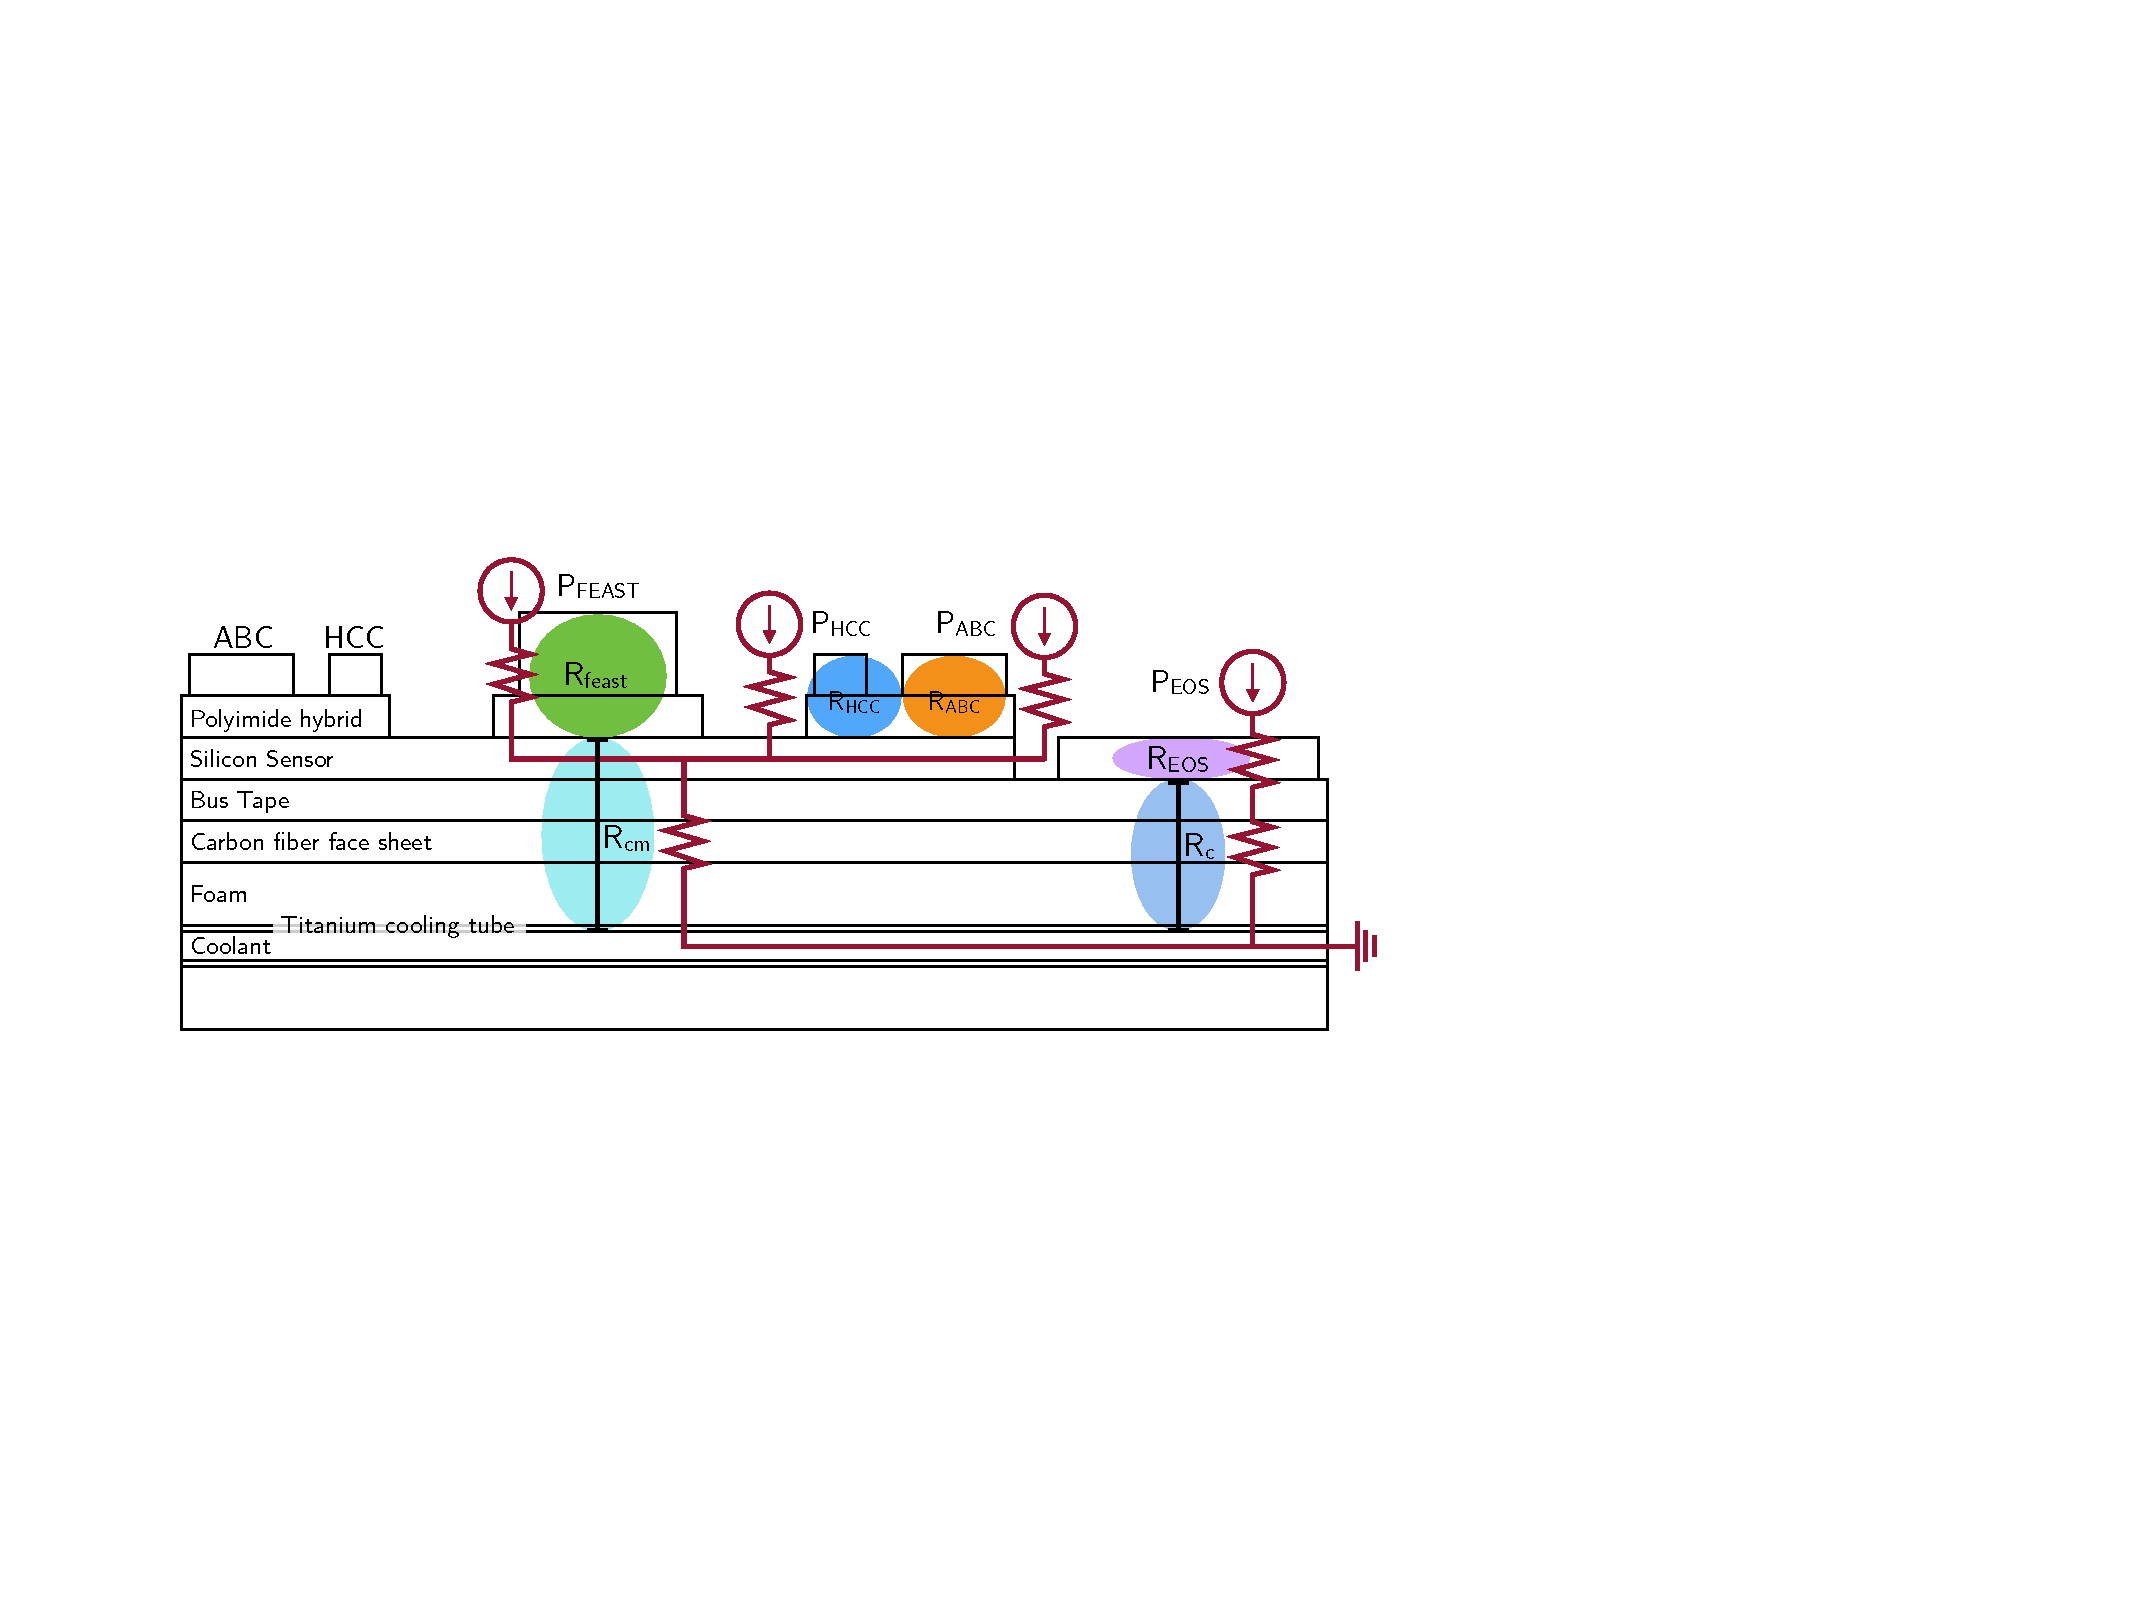
\includegraphics[width=.99\textwidth]{figures/thermoelectric_model.pdf}
\caption{
The thermo-electric model, its analogy with electrical circuits, and definitions of terms.
}
\label{thermoelectric_model}
\end{figure}

Note that e.g. all ABCs are treated as a single node in this description, meaning the ABC power refers
to the total power in all ABCs, and the thermal resistance is an effective thermal resistance for all
ABCs (the same applies to the FEAST and HCC).

Note that the effect of the AMAC as a power source affecting the module temperature is neglected in
the following; however, the AMAC represents roughly 1\% of the total module power, so the impact on
the temperatures of the module is negligible. (The AMAC power itself is counted as part of the total
module power.)

The pathway shared by the EOS and the other components is called $R_{C}$, and is also fit using the
data by measuring the temperature. The two are related according to $R_{CM} = R_C + R_M$.

%\clearpage

\section{Layout of the Endcap Petal}

Figure~\ref{endcap_model} depicts the endcap petal model used for calculating thermal impedances.

\begin{figure}[ht!]
\begin{center}
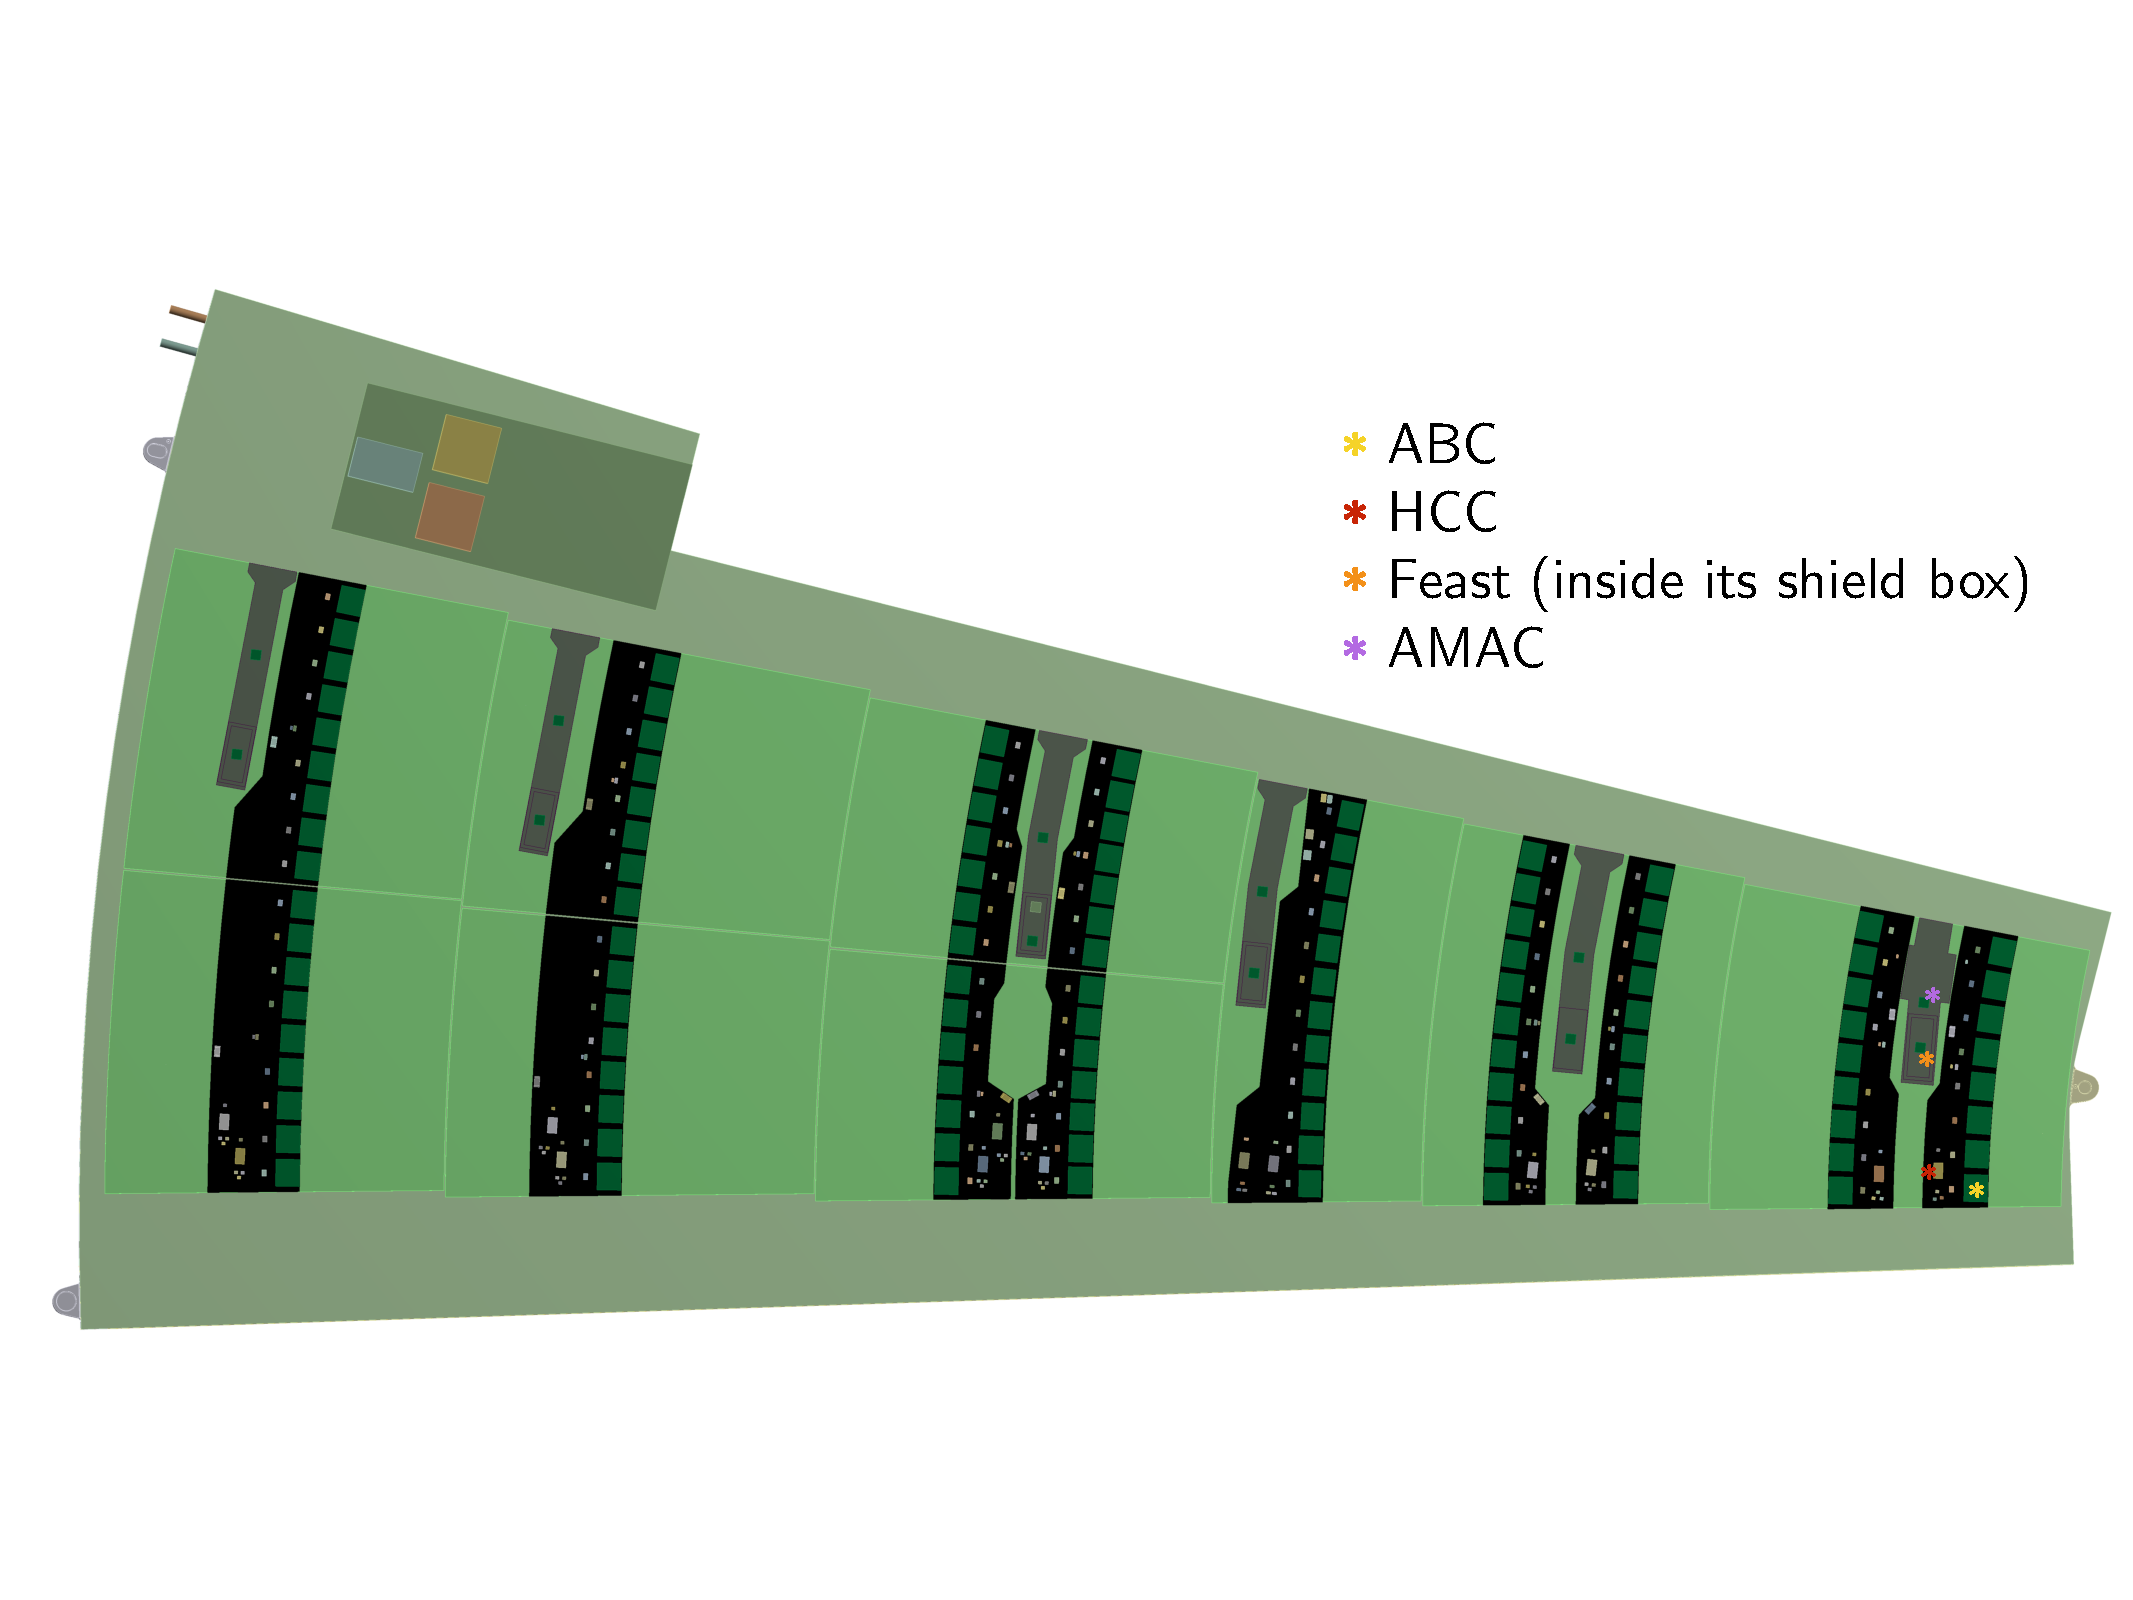
\includegraphics[width=0.99\linewidth]{figures/m30C_0Wm2C_Setup.pdf}
\end{center}
\caption{The endcap petal model used for extracting thermal impedances. The front-end components are
labeled in R1 (the rightmost module).}
\label{endcap_model}
\end{figure}

The number of FEASTs, AMACs, ABCs, HCC, and the sensor area of each module are listed in
Table~\ref{tab:layout_parameters}.
%
\let\arraystretcha\arraystretch
\renewcommand\arraystretch{1.1} % 1.6
\begin{table}[h]
\begin{center}
\adjustbox{max width=\textwidth}{ %% just before tabular
\begin{tabular}{|l|r|r|r|r|r|r|} \hline
Module & nFeast & nAMAC & nABC & nHCC & Sensor area (cm$^2$) \\ \hline
R0     &      1 &     1 &   17 &    2 &                 92.0 \\
R1     &      1 &     1 &   21 &    2 &                 91.0 \\
R2     &      1 &     1 &   12 &    2 &                 76.0 \\
R3     &      2 &     2 &   28 &    4 &                164.0 \\
R4     &      1 &     1 &   16 &    2 &                178.0 \\
R5     &      1 &     1 &   18 &    2 &                186.0 \\
\hline \end{tabular}
} %% resizebox after tabular
\end{center}
\caption{Number of components on each module.}
\label{tab:layout_parameters}
\end{table}
\let\arraystretch\arraystretcha


%\clearpage

\clearpage

\newcommand{\highlight}[1]{{\color{BrickRed}\textbf{#1}}}

\section{Power Inputs for the Endcap Petal Model}

Table~\ref{tab:power_numbers} details the current, voltage, and power specifications for each
front-end component. The values should match the numbers used in the barrel thermal model.

\def\tid{\ensuremath{^*\xspace}}
\def\eff{\ensuremath{\varepsilon}}
\def\pfeast{\ensuremath{\frac{(1-\eff)}{\eff}(P_\text{ABC}+P_\text{HCC})}}
%
\let\arraystretcha\arraystretch
\renewcommand\arraystretch{1.2} % 1.6
\begin{table}[h!]
\begin{center}
\adjustbox{max width=\textwidth}{ %% just before tabular
\begin{tabular}{|l|c|c|c|c|c|c|c|} \hline
\multirow{2}{*}{Description} & input voltage & \multicolumn{4}{c|}{Specifications for 1 component} & $n$ components & Total power \\
              & [V]           & current [A] &\% bumped & power [W]                   & eff   & per module (1 side) & (1 side) [W] \\ \hline
AMAC 1.5V     & 1.5           & 0.042               &  & 0.063                       &       & --                  &       \\
AMAC 2.5V     & 2.5           & 0.002               &  & 0.005                       &       & --                  &       \\
Total AMAC    & --            & --                  &  & \color{blue}{0.068}         &       & R3: 2               & 0.136 \\
              &               &                     &  &                             &       & All others: 1       & 0.068 \\ \hline
ABC (digital) & 1.5           & 0.027          & 110\% & 0.0405                      &       & --                  &       \\
ABC (analog)  & 1.5           & 0.068               &  & 0.102                       &       & --                  &       \\
Total ABC     & --            & 0.095               &  & \color{blue}{0.1425}\tid    &       & R0: 17              & 2.423 \\
              &               &                     &  &                             &       & R1: 21              & 2.993 \\
              &               &                     &  &                             &       & R2: 12              & 1.710 \\
              &               &                     &  &                             &       & R3: 28              & 3.990 \\
              &               &                     &  &                             &       & R4: 16              & 2.280 \\
              &               &                     &  &                             &       & R5: 18              & 2.565 \\ \hline
HCC (digital) & 1.5           & 0.210         & 25.5\% & 0.315                       &       & --                  &       \\
HCC (analog)  & 1.5           & 0.0                 &  & 0.0                         &       & --                  &       \\
Total HCC     & --            & 0.210               &  & \color{blue}{0.315}\tid     &       & R3: 4               & 1.260 \\
              &               &                     &  &                             &       & All others: 2       & 0.630 \\ \hline
bPOL12V (ABC,HCC,AMAC1.5) & --&                     &  & \pfeast   \tid              & 72\%  & --                  & R0: \color{blue}{1.187} \\
              &               &                     &  &                             &       &                     & R1: \color{blue}{1.409} \\
              &               &                     &  &                             &       &                     & R2: \color{blue}{0.910} \\
              &               &                     &  &                             &       &                     & R3: \color{blue}{1.021+1.021} \\
              &               &                     &  &                             &       &                     & R4: \color{blue}{1.132} \\
              &               &                     &  &                             &       &                     & R5: \color{blue}{1.243} \\ \hline
linPOL12V (for AMAC2.5) & --  &                     &  & see text                    &       & --                  & R3: \color{blue}{0.450 + 0.450} \\
              &               &                     &  &                             &       & --                  & All others: \color{blue}{0.450} \\ \hline
Total Module  & --            &                     &  & \tid                        &       &                     & R0: 4.758 \\
              &               &                     &  &                             &       &                     & R1: 5.549 \\
              &               &                     &  &                             &       &                     & R2: 3.768 \\
              &               &                     &  &                             &       &                     & R3: 8.328 \\
              &               &                     &  &                             &       &                     & R4: 4.560 \\
              &               &                     &  &                             &       &                     & R5: 4.956 \\ \hline
\multicolumn{8}{|c|}{} \\[-2mm]
\multicolumn{8}{|c|}{EOS} \\ \hline
lpGBT                     & 1.2         & 0.317     &  & 0.380                       &       & --                  & \color{blue}{0.380} \\ \hline
VTRx (VL+) GBLD 1.2V      & 1.2         & 0.025     &  & 0.030                       &       & --                  & \\
VTRx (VL+) GBLD 2.5V      & 2.5         & 0.07      &  & 0.175                       &       & --                  & \\
VTRx (VL+) GBTIA (legacy) & 2.5         & 0.053     &  & 0.133                       &       & 1                   & \\
Total VTRx (VL+)          &             &           &  & 0.338                       &       & 1                   & \color{blue}{0.338} \\ \hline
bPOL2V5 (old DCDC2)       &             &           &  &                             & 88\%  & 2$\times$, master only         & \color{blue}{0.056+0.056} \\
bPOL12V       &               &                     &  &                             & 55\%  & 2$\times$, master only         & \color{blue}{0.633+0.633} \\ \hline
EOS Master    &               &                     &  &                             &       &                     & 2.096 \\
EOS Slave     &               &                     &  &                             &       &                     & 0.718 \\
EOS both sides&               &                     &  &                             &       &                     & 2.814 \\
\hline \end{tabular}
} %% resizebox after tabular
\end{center}
\caption{Endcap module inputs.
Values with \tid~next to them are affected by the TID bump in one way or another. The bPOL12V efficiency
is representative only; in reality it is temperature- and current-dependent.
Note that there are two bPOL12V converters and two linPOL12V converters on R3.
Further notes are
described in the text.
}
\label{tab:power_numbers}
\end{table}
\let\arraystretch\arraystretcha

Some notes on the numbers in the table:
\begin{itemize}
\item HCC and ABC power numbers correspond to unirradiated values.
\item Items marked with a ``\tid'' are affected by the digital current increase caused by the TID.
The bPOL12V is affected by the TID bump insofar as its power is determined by the ABC and HCC.
%% \item In the ABC, we have 42.5~mA digital with a 69\% bump, plus 70~mA analog. This is equivalent to
%% 29~mA fully bumped, and 83~mA non-bumped current. (Old values.)
\item The HCC is assumed to have a smaller TID bump than the ABC. This is accounted by an additional
scaling for the HCC case - see Section~\ref{tid_parameterization_details}. But because this scaling
is functionally the same as the ABC bump fraction, we write it here as well.
\item In the above, the bPOL12V efficiency is assumed to be constant, but in reality it is temperature- and
current-dependent.
\item In the EOS, the bPOL12V has a lower efficiency than in the module because the current load is
much smaller, and the bPOL12V is much less efficient in this regime.
\item The total module power (before irradiation, before TID bump) in the table represents
all components excluding HV and tape losses, which are small in comparison.
\end{itemize}

\noindent
Comments on the EOS components:

\begin{itemize}
%% \item For the EOS, the total power for both sides is simply double the power of one side.
\item The EOS bPOL12Vs and bPOL2V5s (was DCDC2) exist on one side only, and power the EOS cards on both petal
sides. There are two of each (one per side). Therefore the EOS numbers are split into ``master'' and ``slave'' numbers.
%% \item For $n=1$ lpGBTx ASICs (corresponding to the barrel long strips and the endcaps),
%% and assuming a BPOL12V efficiency $\varepsilon_\text{BPOL12V}=0.75$,
%% the total power is 1.4~W per EOS side.
%% \item For $n=2$ lpGBTx ASICs (corresponding to the barrel short strips), the total power is 2.6~W per
%% EOS side.
\end{itemize}

%% \subsection{The End-of-Substructure (EOS)}
%% \begin{itemize}
%% \item DCDC2 converter: $P=0.208$~W (see calculation below)
%% \item BPOL12V: $P=1.12$~W (see calculation below)
%% \item VTRx
%%   \begin{itemize}
%%     \item GBTIA: $I=53$~mA; 2.5~V; $P=0.1325$~W
%%     \item GBLD$_{2.5V}$: $I=18$~mA 2.5~V; $P=0.045$~W
%%   \end{itemize}
%% \item lpGBTx: $I=625$~mA; 1.2~V; $P=0.75$~W; powered by DCDC2
%% \item GBLD$_{1.2V}$: $I=9.5$~mA; 1.2~V; $P=0.0114$~W; powered by DCDC2
%% \end{itemize}

\subsection{Power Equations for the EOS, bPOL12V, bPOL2V5 and linPOL12V}

The total power of the EOS (one side) is given by:
\begin{equation}
P_\text{EOS} = \frac{1}{\varepsilon_\text{bPOL12V}}\times
  \left( \frac{1}{\varepsilon_\text{bPOL2V5}} (n P_\text{lpGBTx} + n P_\text{GBLD1.2}) + n P_\text{GBLD2.5} + P_\text{GBTIA} \right)
\end{equation}
% (((.750*2+0.0114*2)/0.88)+0.1325+0.045*2)/0.75 = 2.60
% (((.750*1+0.0114*1)/0.88)+0.1325+0.045*1)/0.75 = 1.40

As can probably be inferred from above, the power attributed to the EOS bPOL12V is:
\begin{equation}
P^\text{EOS}_\text{bPOL12V} = \frac{(1-\varepsilon_\text{bPOL12V})}{\varepsilon_\text{bPOL12V}}\times
  \left( \frac{1}{\varepsilon_\text{bPOL2V5}} (n P_\text{lpGBTx} + n P_\text{GBLD1.2}) + n P_\text{GBLD2.5} + P_\text{GBTIA} \right)
\end{equation}

The power in the EOS bPOL2V5 (was called DCDC2) converter is:
\begin{equation}
P^\text{EOS}_\text{bPOL2V5} = \frac{(1-\varepsilon_\text{bPOL2V5})}{\varepsilon_\text{bPOL2V5}} \left(n P_\text{lpGBTx} + n P_\text{GBLD1.2}\right)
\end{equation}


The power dissipated by the linPOL12V (powering the AMAC) is given by the current in the AMAC components
(adding the quiescent current, 1.9 mA) multiplied by the voltage drop in the linPOL12V:
\begin{equation}
P_\text{linPOL12V} = (I^{1.5V}_\text{AMAC} + I^\text{q}_\text{linPOL12V})\left(  \Delta V_\text{linPOL12V} - 1.5V \right)
                   + (I^{3.0V}_\text{AMAC} + I^\text{q}_\text{linPOL12V})\left(  \Delta V_\text{linPOL12V} - 3.0V \right)
\label{eq:amac_regulator}
\end{equation}
where the calculation of $\Delta V_\text{linPOL12V}$ is described in Section~\ref{low_voltage}.

\subsection{bPOL12V (FEAST) efficiency}

The bPOL12V efficiency varies as a function of temperature and load current. The parameterization used
is the one derived by Georg. Figure~\ref{feast_vs_temperature} highlights the agreement between the
measured FEAST efficiencies and the parameterized fit.

\begin{figure}[ht!]
\begin{center}
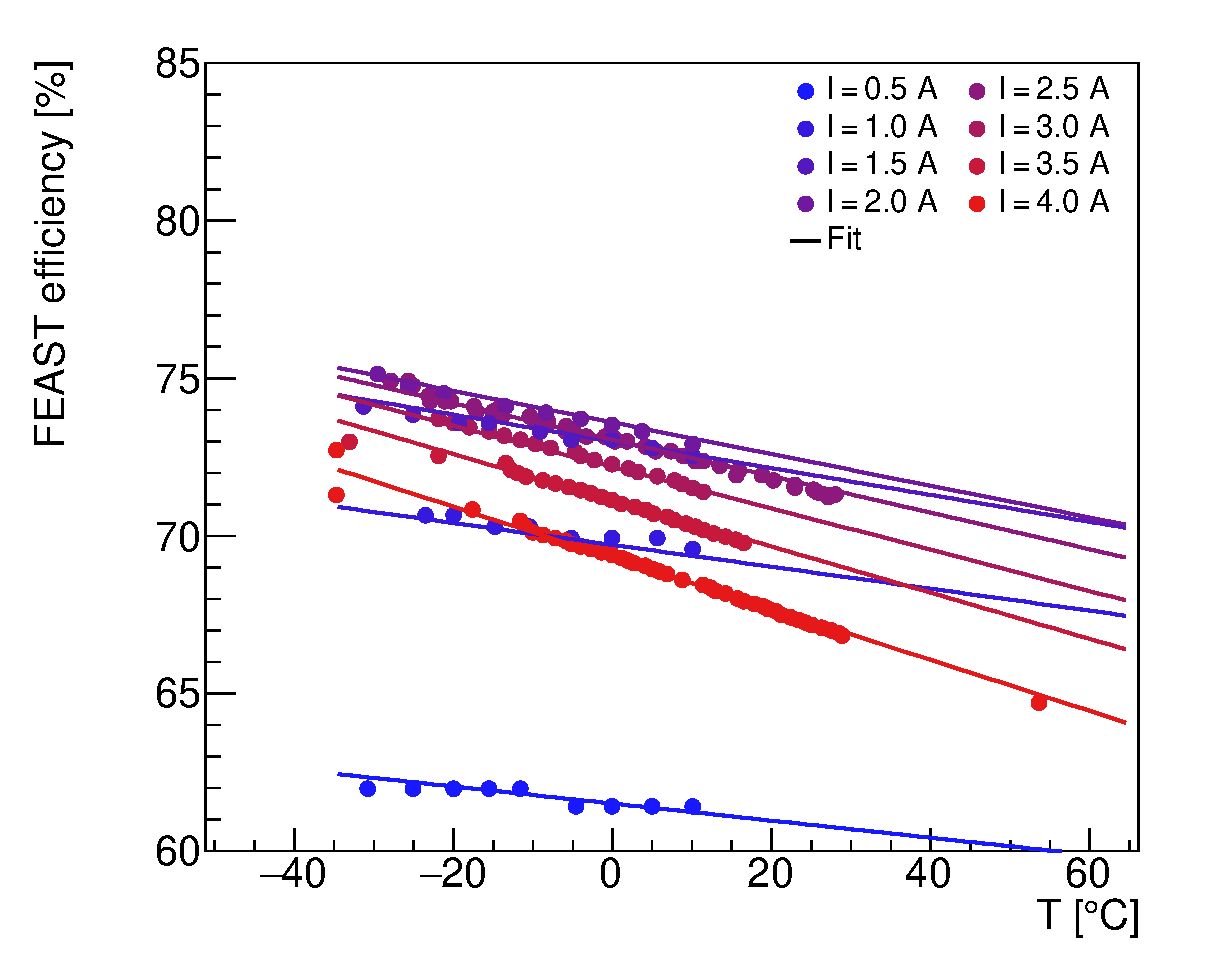
\includegraphics[width=0.49\linewidth]{figures/FeastEfficiency_isoCurrent}
\end{center}
\caption{FEAST efficiency data versus temperature ($x$-axis) and current (indicated with different
colors). The parameterization of the data is represented by the fit lines at fixed current.
}
\label{feast_vs_temperature}
\end{figure}

\subsection{TID bump parameterization}
\label{tid_parameterization_details}

The TID bump parameterization is the one supplied by Kyle Cormier for the ABC130$^{*}$
(Nominal parameters: $a=1.402\times 10^{11}$, $b=-1.62$.
Pessimistic parameters: $a=2.64\times10^{9}$, $b=-1.35$.)
Figure~\ref{tid_parameterization} shows the TID parameterization used in the current model. This
parameterized bump is applied to the ``bumped'' fraction of digital current, as indicated in
Table~\ref{tab:power_numbers}.

\begin{figure}[ht!]
\begin{center}
\begin{subfigure}[t]{0.49\textwidth}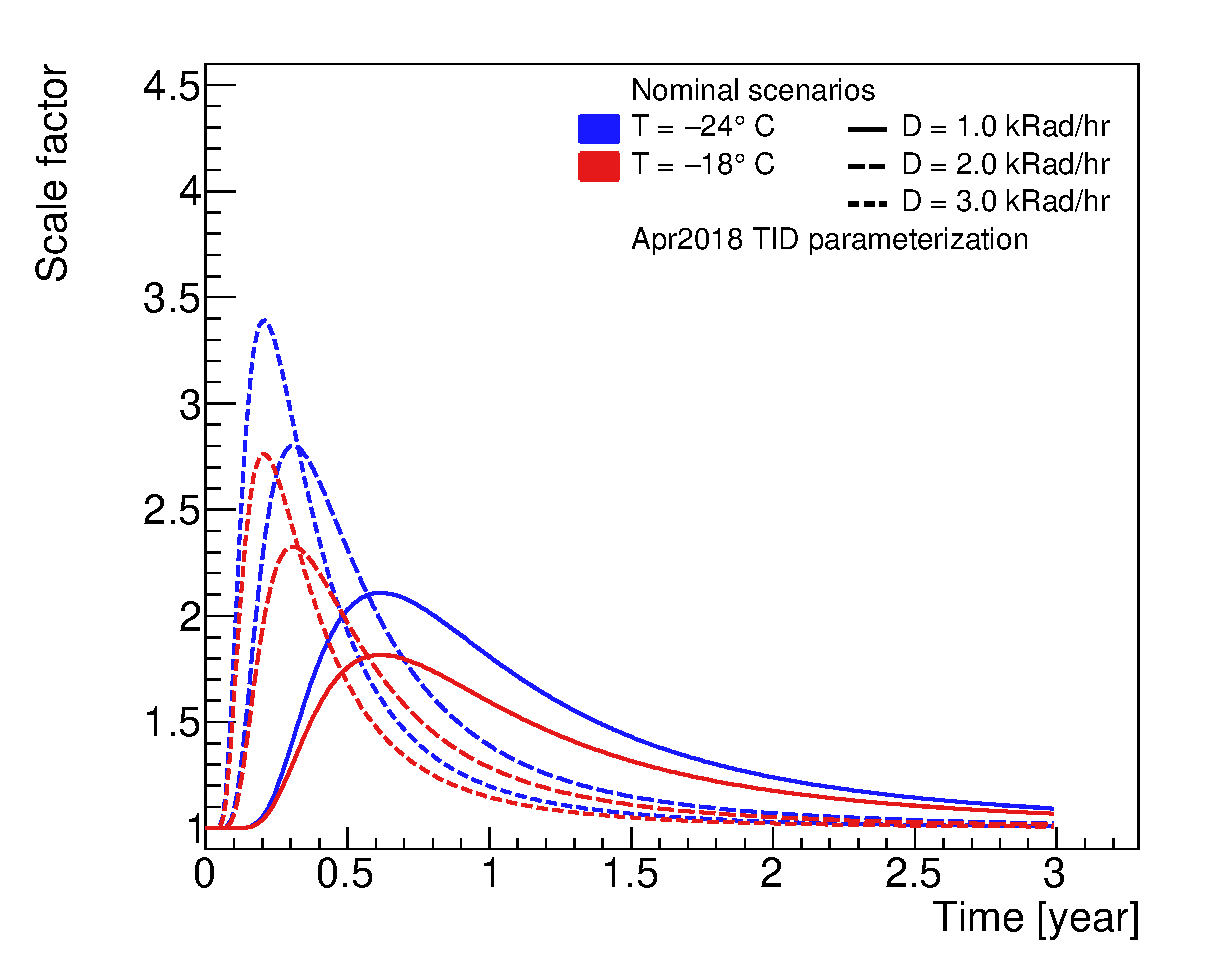
\includegraphics[width=0.99\linewidth]{figures/AbcTidBumpVersionRatesAndTemps_Nominal}\caption{Nominal Case}\end{subfigure}
\begin{subfigure}[t]{0.49\textwidth}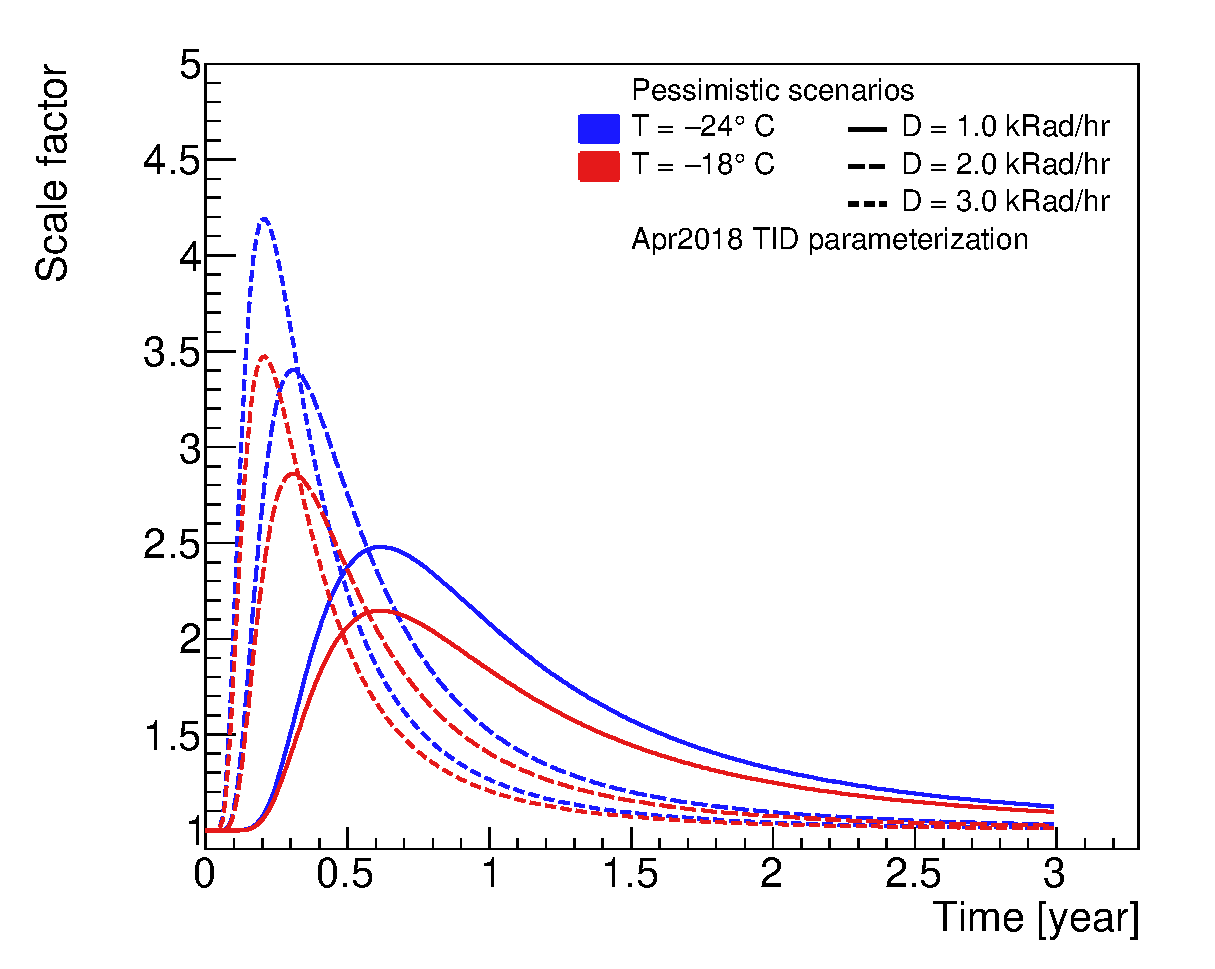
\includegraphics[width=0.99\linewidth]{figures/AbcTidBumpVersionRatesAndTemps_Pessimistic}\caption{Pessimistic Case}\end{subfigure}
\end{center}
\caption{TID parameterization vs time, for two representative temperatures (indicated by
color) and three dose rates (indicated by line style). Nominal and Pessimistic cases are shown.}
\label{tid_parameterization}
\end{figure}

\subsubsection*{HCC Treatment}

The HCC is assumed to have a smaller TID bump than the ABC. Thus, the HCC TID bump
is scaled by a factor (see Table~\ref{tab:power_numbers}) to account for the smaller observed HCC TID bump.

\subsection{Summary of Power Contributions in R1}

A stack plot showing the contributions of each component to the total power is shown in
Figure~\ref{power_stackplot}.

\begin{figure}[ht!]
\begin{center}
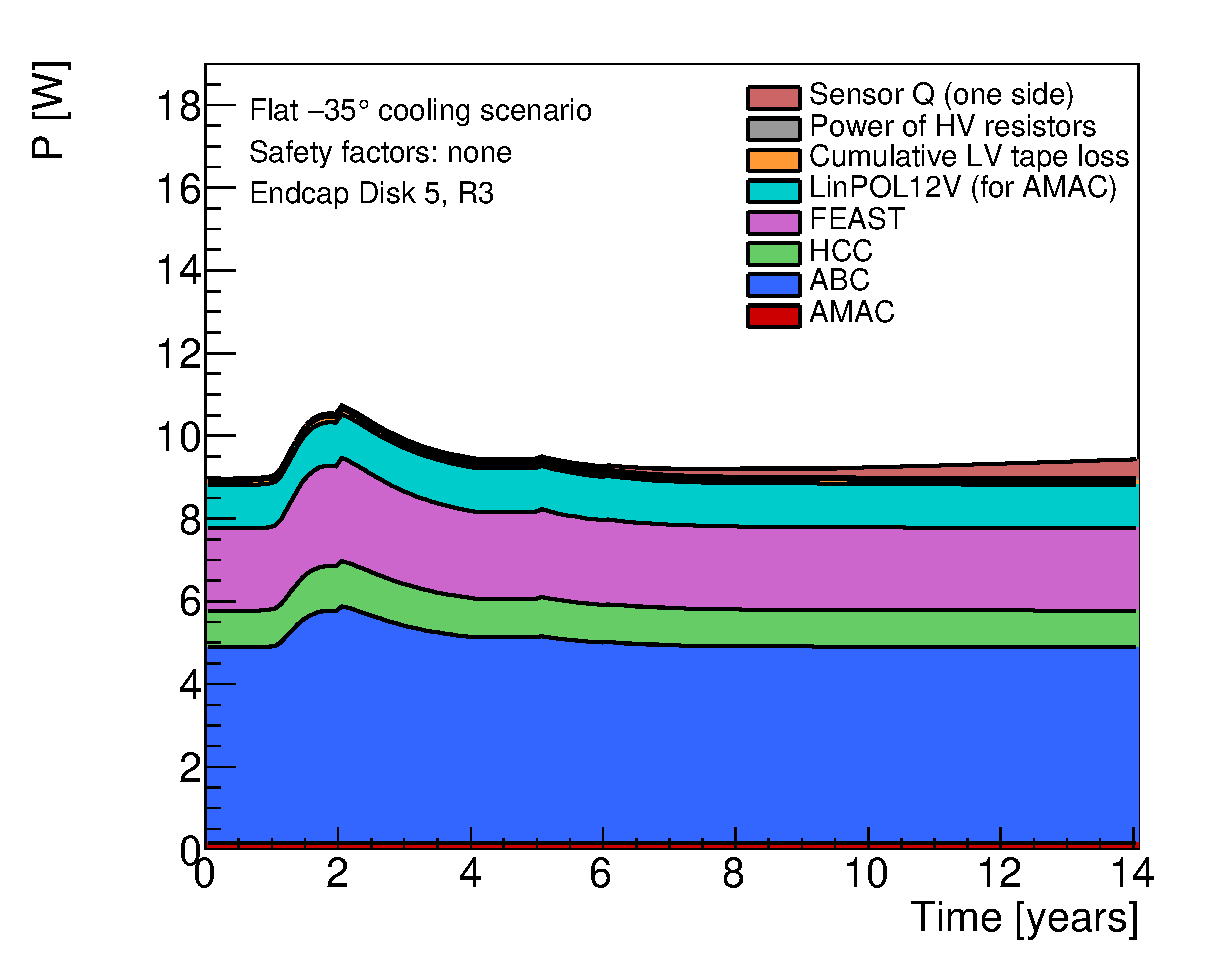
\includegraphics[width=0.55\linewidth]{figures/PowerStackPlot.eps}
\end{center}
\caption{Summary of the contributions of each front-end component to the total power in R3 (Disk 5), given
a nominal TID bump parameterization and no safety factors, to illustrate the relative contributions
of each component.}
\label{power_stackplot}
\end{figure}


\clearpage

\newcommand{\highlight}[1]{{\color{BrickRed}\textbf{#1}}}

\section{Collecting Power Inputs for the Endcap Petal}

Table~\ref{tab:power_numbers} details the current, voltage, and power specifications for each
component. Most of these numbers come from Graham and Georg's thermal model. Most are similar to
Sergio's numbers, with some differences highlighted in red.

\def\tid{\ensuremath{^\text{TID}}\xspace}
\def\eff{\ensuremath{\varepsilon}}
\def\pfeast{\ensuremath{\frac{(1-\eff)}{\eff}(P_\text{ABC}+P_\text{HCC})}}
%
\let\arraystretcha\arraystretch
\renewcommand\arraystretch{1.2} % 1.6
\begin{table}[h]
\begin{center}
\adjustbox{max width=\textwidth}{ %% just before tabular
\begin{tabular}{|l|c|c|c|c|c|c|} \hline
\multirow{2}{*}{Description} & input voltage & \multicolumn{3}{c|}{Specifications for 1 component} & $n$ components & Total power \\
              & [V]           & current [A]           & power [W]                   & eff   & per module (1 side) & (1 side) [W]    \\ \hline
AMAC 1.5V     & 1.5           & 0.045                 & 0.0675                      &       & --                  &                 \\
AMAC 3.0V     & 3.0           & 0.002                 & 0.006                       &       & --                  &                 \\
Total AMAC    & --            & --                    & 0.0735                      &       & 1                   & 0.0735          \\ \hline
ABC (digital) & 1.5           & 0.035                 & 0.0525                      &       & --                  &                 \\
ABC (analog)  & 1.5           & 0.066                 & 0.099                       &       & --                  &                 \\
Total ABC     & --            & 0.101                 & 0.1515                      &       & 21$^*$              & 3.1815$^*$\tid  \\ \hline
HCC (digital) & 1.5           & 0.125                 & 0.1875                      &       & --                  &                 \\
HCC (analog)  & 1.5           & 0.075                 & 0.1125                      &       & --                  &                 \\
Total HCC     & --            & 0.200                 & 0.3                         &       & 2$^*$               & 0.6$^*$\tid     \\ \hline
FEAST (ABC,HCC) & --          &                       & \pfeast                     & 75\%  & --                  & 1.2605$^*$\tid  \\
``FEAST'' AMAC regulators & --&                       & see below                   &       & --                  & 0.415           \\
Total FEAST   & --            &                       & see below                   &       & 1                   & 1.6755$^*$\tid  \\ \hline
Total Module (R1)  & --       &                       &                             &       &                     & 5.53$^*$        \\ \hline
\multicolumn{7}{|c|}{} \\[-2mm]
\multicolumn{7}{|c|}{EOS} \\ \hline
VTRx: lpGBTx  & 1.2           & 0.625                 & 0.750                       &       & --                  &                 \\
VTRx: GBLD 1.2V & 1.2         & 0.0095                & 0.0114                      &       & --                  &                 \\
VTRx: GBLD 2.5V & 2.5         & 0.018                 & 0.045                       &       & --                  &                 \\
Total VTRx    &               &                       & 0.8064                      &       & 1                   & 0.8064          \\         
GBTIA         & 2.5           & 0.053                 & 0.1325                      &       & 1                   & 0.1325          \\
FEAST         &               &                       &                             &       & 0.5$^\dagger$       & 0.35$^\dagger$  \\
DCDC2         &               &                       &                             & 88\%  & 0.5$^\dagger$       & 0.104$^\dagger$ \\ \hline
Total EOS     &               &                       &                             &       &                     & 1.4             \\
EOS both sides&               &                       &                             &       &                     & 2.8             \\
\hline \end{tabular}
} %% resizebox after tabular
\end{center}
\caption{Endcap module inputs. Starred ($^*$) values are representative and taken from Endcap R1. Values
with \tid next to them are affected by the TID bump in one way or another. The 75\% FEAST efficiency 
is representative only; in reality it is temperature- and current-dependent (also TID-dependent?).
}
\label{tab:power_numbers}
\end{table}
\let\arraystretch\arraystretcha

Some notes on the numbers in the table:
\begin{itemize}
\item HCC and ABC power numbers correspond to unirradiated values.
\item The ABC power numbers (from Georg/Graham) differ from Sergio's sheet by 1.7\%.
\item \highlight{The HCC power numbers (from Georg/Graham) differ from Sergio's sheet by 38\%.}
\item \tid The FEAST is affected by the TID bump insofar as its power is determined by the ABC and HCC.
  In the above it is assumed to be 75\%, but it is temperature and current-dependent.
\item The total power (before irradiation, before TID bump) of Module R1 represents
all components excluding HV and tape losses, which are small in comparison.
\item For the EOS, the total power for both sides is simply double the power of one side.
\item $^\dagger$ The FEAST and DCDC2 exist on one side only, and power the EOS cards on both petal
sides (hence ``0.5 per side''). If both EOSes are powered, then the power dissipatd by the FEAST and
DCDC2 is twice the power listed above.
\item For $n=1$ lpGBTx ASICs (corresponding to the barrel long strips and the endcaps),
and assuming a FEAST efficiency $\varepsilon_\text{FEAST}=0.75$,
the total power is 1.4~W per EOS side.
\item For $n=2$ lpGBTx ASICs (corresponding to the barrel short strips),
\highlight{the total power is 2.6~W per EOS side (differs from the TDR, which says 3~W)}.
\end{itemize}

%% \subsection{The End-of-Substructure (EOS)}
%% \begin{itemize}
%% \item DCDC2 converter: $P=0.208$~W (see calculation below)
%% \item FEAST: $P=1.12$~W (see calculation below)
%% \item VTRx
%%   \begin{itemize}
%%     \item GBTIA: $I=53$~mA; 2.5~V; $P=0.1325$~W
%%     \item GBLD$_{2.5V}$: $I=18$~mA 2.5~V; $P=0.045$~W
%%   \end{itemize}
%% \item lpGBTx: $I=625$~mA; 1.2~V; $P=0.75$~W; powered by DCDC2
%% \item GBLD$_{1.2V}$: $I=9.5$~mA; 1.2~V; $P=0.0114$~W; powered by DCDC2
%% \end{itemize}

The total power of the EOS (one side) is given by:
\begin{equation}
P_\text{EOS} = \frac{1}{\varepsilon_\text{FEAST}}\times
  \left( \frac{1}{\varepsilon_\text{DCDC2}} (n P_\text{lpGBTx} + n P_\text{GBLD1.2}) + n P_\text{GBLD2.5} + P_\text{GBTIA} \right)
\end{equation}
% (((.750*2+0.0114*2)/0.88)+0.1325+0.045*2)/0.75 = 2.60
% (((.750*1+0.0114*1)/0.88)+0.1325+0.045*1)/0.75 = 1.40

As can probably be inferred from above, the power in the EOS FEAST is:
\begin{equation}
P^\text{EOS}_\text{FEAST} = \frac{(1-\varepsilon_\text{FEAST})}{\varepsilon_\text{FEAST}}\times
  \left( \frac{1}{\varepsilon_\text{DCDC2}} (n P_\text{lpGBTx} + n P_\text{GBLD1.2}) + n P_\text{GBLD2.5} + P_\text{GBTIA} \right)
\end{equation}

The power in the EOS DCDC2 converter is:
\begin{equation}
P^\text{EOS}_\text{DCDC2} = \frac{(1-\varepsilon_\text{DCDC2})}{\varepsilon_\text{DCDC2}} \left(n P_\text{lpGBTx} + n P_\text{GBLD1.2}\right)
\end{equation}


The power dissipated by the AMAC regulators is given by the current in the AMAC components multiplied
by the voltage drop in the regulators:
\begin{equation}
P_\text{regulator} = I^{1.5V}_\text{AMAC}\left(  10.5V - 1.5V \right)
                   + I^{3.0V}_\text{AMAC}\left(  10.5V - 3.0V \right)
\label{eq:amac_regulator}
\end{equation}



\section{ Extracting thermal impedances using FEA simulations}

\subsection{Setup of the FEA Simulation to extract thermal impedances}

Representative power numbers are used to power each component. In each simulation run, all instances
of one type of component (e.g. the ABCs) are powered on in all six modules, keeping the rest off.
Average temperatures are measured for the following components (see below): HCC, ABC, FEAST, sensor.

\def\thcc{\ensuremath{\overline{T}_\text{nHCC}}}
\def\tabc{\ensuremath{\overline{T}_\text{nABC}}}
\def\tfeast{\ensuremath{\overline{T}_\text{FEAST}}}
\def\tsensor{\ensuremath{T_\text{sensor}}}
\def\Rm{\ensuremath{{\text{R}m}}}

\begin{itemize}
\item FEAST: a $3\times3$~mm $\times~350~\mu$m chip inside the shield box.
  \begin{itemize}
  \item The FEAST has an additional power term due to regulators for the AMAC -- see below.
  \end{itemize}
\item AMAC: a $3\times3$~mm $\times~350~\mu$m chip, roughly in the center of the power board
  \begin{itemize}
    \item The AMAC is powered using regulators located in the FEAST chip, with a power dissipation
      of the regulators corresponding to the voltage drop in the regulator (0.415~W) -- see Eq.~\ref{eq:amac_regulator}.
  \end{itemize}
\item HVMUX: Ignore for now
\item EOS (\highlight{3.20~W total, including both sides -- see Table~\ref{tab:power_numbers}.}) % (\highlight{3.03~W total, for both sides}):
  \begin{itemize}
  \item \highlight{Placement of these EOS power sources: ???}
%%     \item 1 lpGBT per side (\highlight{0.750~W $\times$ 2 sides})
%%     \item ``Rest'' (1 VTRX optical link per side?) (\highlight{.185~W $\times$ 2 sides}) ???
%%     \item FEAST on a single side (\highlight{1.12~W})
%%     \item DCDC2 converter on a single side (\highlight{0.21~W})
  \end{itemize}
\item Cooling: Constant 8000~W/m$^{2}$K, $-30$~C, no convection
\end{itemize}




\subsection{FEA Simulation Runs to extract thermal impedances}

For the extraction of the thermal impedances, a simplified set of input power parameters are used,
summarized in Table~\ref{tab:simulation_runs}.
In the FEA, the power is distributed over all 6 surfaces (\highlight{different from barrel treatment}).

\let\arraystretcha\arraystretch
\renewcommand\arraystretch{1.4} % 1.6
\begin{table}[h!]
\footnotesize
\begin{center}
\adjustbox{max width=\textwidth}{ %% just before tabular
\begin{tabular}{|l|l|l|l|} \hline
Simulation \# & Description                        & Input parameters           \\ \hline
1             & All HCCs powered on, rest off      & $P_\text{HCC}=0.413$~W     \\
2             & All ABCs powered on, rest off      & $P_\text{ABC}=0.149$~W     \\
3             & All FEASTs powered on, rest off    & $P_\text{FEAST}=1.5$~W$^*$ \\ \hline
\multicolumn{3}{|c|}{Extended simulations} \\ \hline
4             & Tape ``powered'' on, rest off      & skip for now \\
5             & HVMUX powered on, rest off         & skip for now \\
6             & R$_\text{HV}$ powered on, rest off & skip for now \\
7             & EOS                                & skip for now \\ % $P_\text{EOS}=3.03$~W$^{**}$
\hline \end{tabular}
} %% resizebox after tabular
\end{center}
\caption{ Description of the 7 thermal simulations required to obtain the thermal impedances.
}
\label{tab:simulation_runs}
\end{table}
\let\arraystretch\arraystretcha

$^*$ The actual nominal power of the FEAST varies for each module; however, for the simulation to extract
the thermal impedances, the power is set to 1.5~W for all FEASTs in the petal.\\






\subsection{Measurements performed in each run}

%% For each component, the temperature measured is the average of the top surface nodes of all
%% components of a given type, in a given module.

The average, min and max temperatures are taken over the volume of the elements (\highlight{different from barrel treatment}).
There are 45 measurements per simulation run in total.

The average temperatures can be measured either \highlight{on one side of the petal, or as the average of components on both sides 
of the petal}.

\begin{itemize}
\item $(\thcc)_\Rm$: The average HCC temperature of the $n$ HCCs in the module, for each module R$m$ (R0, R1, ... R5) (6~total)
\item $(\tabc)_\Rm$: The average ABC temperature of the $n$ ABCs in the module, for each module R$m$ (6~total)
\item $(\tfeast)_\Rm$: The temperature of the FEAST in the module, for each module R$n$ (6~total)
\item \tsensor, taken for R0, R1, R2, R3\_left, R3\_right, R4\_left, R4\_right, R5\_left, R5\_right (9~total) (27~total measurements):
\begin{itemize}
  \item $\tsensor^\text{Avg}$: The average sensor temperature taken over the volume of the sensor
  \item $\tsensor^\text{Max}$: The maximum sensor temperature in the module, for each module
  \item $\tsensor^\text{Min}$: The minimum sensor temperature in the module, for each module
\end{itemize}
\end{itemize}




\section{The Linear Model}

\subsection{Additional parameters in the linear model}

The number of ABCs, HCC, and the sensor area are below,
as are the FEAST currents before irradiation (pre-TID bump).
%
\let\arraystretcha\arraystretch
\renewcommand\arraystretch{1.1} % 1.6
\begin{table}[h]
\footnotesize
\begin{center}
\adjustbox{max width=\textwidth}{ %% just before tabular
\begin{tabular}{|l|r|r|r|r|r|} \hline
Module & nABC & nHCC & Sensor area (cm$^2$) & $I_\text{FEAST}$ [A] & $P_\text{FEAST}$ \\ \hline
R0     &   17 &    2 &                 92.0 &              2.12 & 1.0585 \\
R1     &   21 &    2 &                 91.0 &              2.52 & 1.2605 \\
R2     &   12 &    2 &                 76.0 &              1.61 & 0.806  \\
R3     &   28 &    4 &                164.0 &              3.63 & 1.814  \\
R4     &   16 &    2 &                178.0 &              2.02 & 1.008  \\
R5     &   18 &    2 &                186.0 &              2.22 & 1.109  \\
\hline \end{tabular}
} %% resizebox after tabular
\end{center}
\caption{Endcap module inputs. The FEAST current is calculated from the HCC and ABC values in
Table~\ref{tab:power_numbers}, and given nABC and nHCC in each module. The FEAST power is calculated
assuming a 75\% efficiency, and does not include the power due to the AMAC regulators.}
\label{tab:spurious_signal_main}
\end{table}
\let\arraystretch\arraystretcha


\subsection{Other assumed quantities}

Assumed quantities are below:
\begin{itemize}
\item $R_\text{EOS}=15.0$~K/W (guessed by Georg/Graham)
\item $R_\text{sensor}=0.02$~K/W (guessed by Georg/Graham)
\item $R_\text{tape}=0.01$~K/W per module (i.e. there are 6 such resistors in the endcap) (worst-case number)
%% \item EOS DCDC2 efficiency: 0.88
%% \item $V_\text{hybrid}=1.5$~V
%% \item $I^\text{digital}_\text{HCC}=0.125$~A (before TID damage; TID-dependent)
%% \item $I^\text{analog}_\text{HCC}=0.075$~A
%% \item $I^\text{digital}_\text{ABC}=0.035$~A (before TID damage; TID-dependent)
%% \item $I^\text{analog}_\text{ABC}=0.066$~A
\end{itemize}

%% The AMAC:
%% \begin{itemize}
%% \item $V^{1.5V}_\text{AMAC} = 1.5$~V
%% \item $I^{1.5V}_\text{AMAC} = 0.045$~A
%% \item (Efficiency $\varepsilon^{1.5V}_\text{AMAC} = 0.65$\% -- not used in model)
%% \item $V^{3.0V}_\text{AMAC} = 3.0$~V
%% \item $I^{3.0V}_\text{AMAC}= 0.002$~A
%% \item (Efficiency $\varepsilon^{3.0V}_\text{AMAC} = 0.65$\% -- not used in model)
%% \end{itemize}

Table~\ref{tab:thermal_impedances} shows the thermal impedances calculated
from the FEA simulations.

\def\insulabc{$R_\text{ABC}\times n_\text{ABC}$\xspace}
\def\insulhcc{$R_\text{HCC}\times n_\text{HCC}$\xspace}

%
\let\arraystretcha\arraystretch
\renewcommand\arraystretch{1.1} % 1.6
\begin{table}[h]
\footnotesize
\begin{center}
\adjustbox{max width=\textwidth}{ %% just before tabular
\begin{tabular}{|l|r|r|r|r|r|r|} \hline
       &                     &                   & \multicolumn{2}{c|}{ABC}   & \multicolumn{2}{c|}{HCC}   \\
Module & $R_\text{cm}$ [K/W] & $ R_\text{FEAST}$ & $R_\text{ABC}$ & \insulabc & $R_\text{HCC}$ & \insulhcc \\ \hline
R0     &               0.802 &            26.045 &          0.917 &    15.589 &         12.632 &    25.264 \\
R1     &               0.991 &            28.256 &          0.671 &    14.091 &         12.744 &    25.488 \\
R2     &               1.410 &            28.883 &          1.550 &    18.600 &         13.794 &    27.588 \\
R3     &               0.873 &            29.333 &          0.566 &    15.848 &          6.812 &    27.248 \\
R4     &               0.744 &            26.816 &          1.432 &    22.912 &         13.027 &    26.054 \\
R5     &               0.690 &            27.450 &          1.034 &    18.612 &         13.177 &    26.354 \\
\hline \end{tabular}
} %% resizebox after tabular
\end{center}
\caption{Effective thermal impedances calculated from Yu-Heng's numbers (in K/W).
For instances where you have $n$ components, the thermal insulance (inverse of HTC) is also calucated, simply
in units of A$_\text{1-device}\cdot$ K/W.
}
\label{tab:thermal_impedances}
\end{table}
\let\arraystretch\arraystretcha

\clearpage

\section{Endcap High Voltage and Sensors in R3-R5}
\label{highvoltage}

The nominal thermoelectric model of an endcap module consists of one sensor connected in parallel with
an HVMUX and in series with a 10~k$\Omega$ filter (technically two 5k resistors).
Note, however, that endcap modules R3, R4 and R5 each contain two sensors, each of which has its own
HVMUX and series resistors. Because leakage current is proportional to the area of a sensor,
the effect of replacing a single sensor with a pair of sensors having the same total area is to split
the leakage current between the two sensors. Therefore, the total leakage current $I_S$ and sensor
power $Q_S$ are the same as in the single-sensor case.

However, these modules have two 10~k$\Omega$ serial resistors, each with half of the total
leakage current, and two HVMUX resistors, meaning the power dissipated is different from the nominal
case:

\begin{align}
P_{RHV}(I_S) ~=~& R_{HV}I_S^2~~\rightarrow~~ 2\times R_{HV}\left(\frac{I_S}{2}\right)^2 \\
P_{HVMUX} ~=~& \frac{ V^2_{bias} }{R_{HVMUX} + R_{HV}} ~~\rightarrow~~ 
             \frac{2V^2_{bias} }{R_{HVMUX} + R_{HV}}.
\end{align}

Thus, when treating the sensors in R3, R4, and R5, thermally the two sensors are treated as one sensor
(see Section~\ref{two_sensors_thermal_treat}, and electrically they are treated as one sensor with the
adjustments described above.


\section{LV and HV Tape, Supply and Cable Losses}

\subsection{Low voltage}
\label{low_voltage}

\begin{figure}[ht!]
\begin{center}
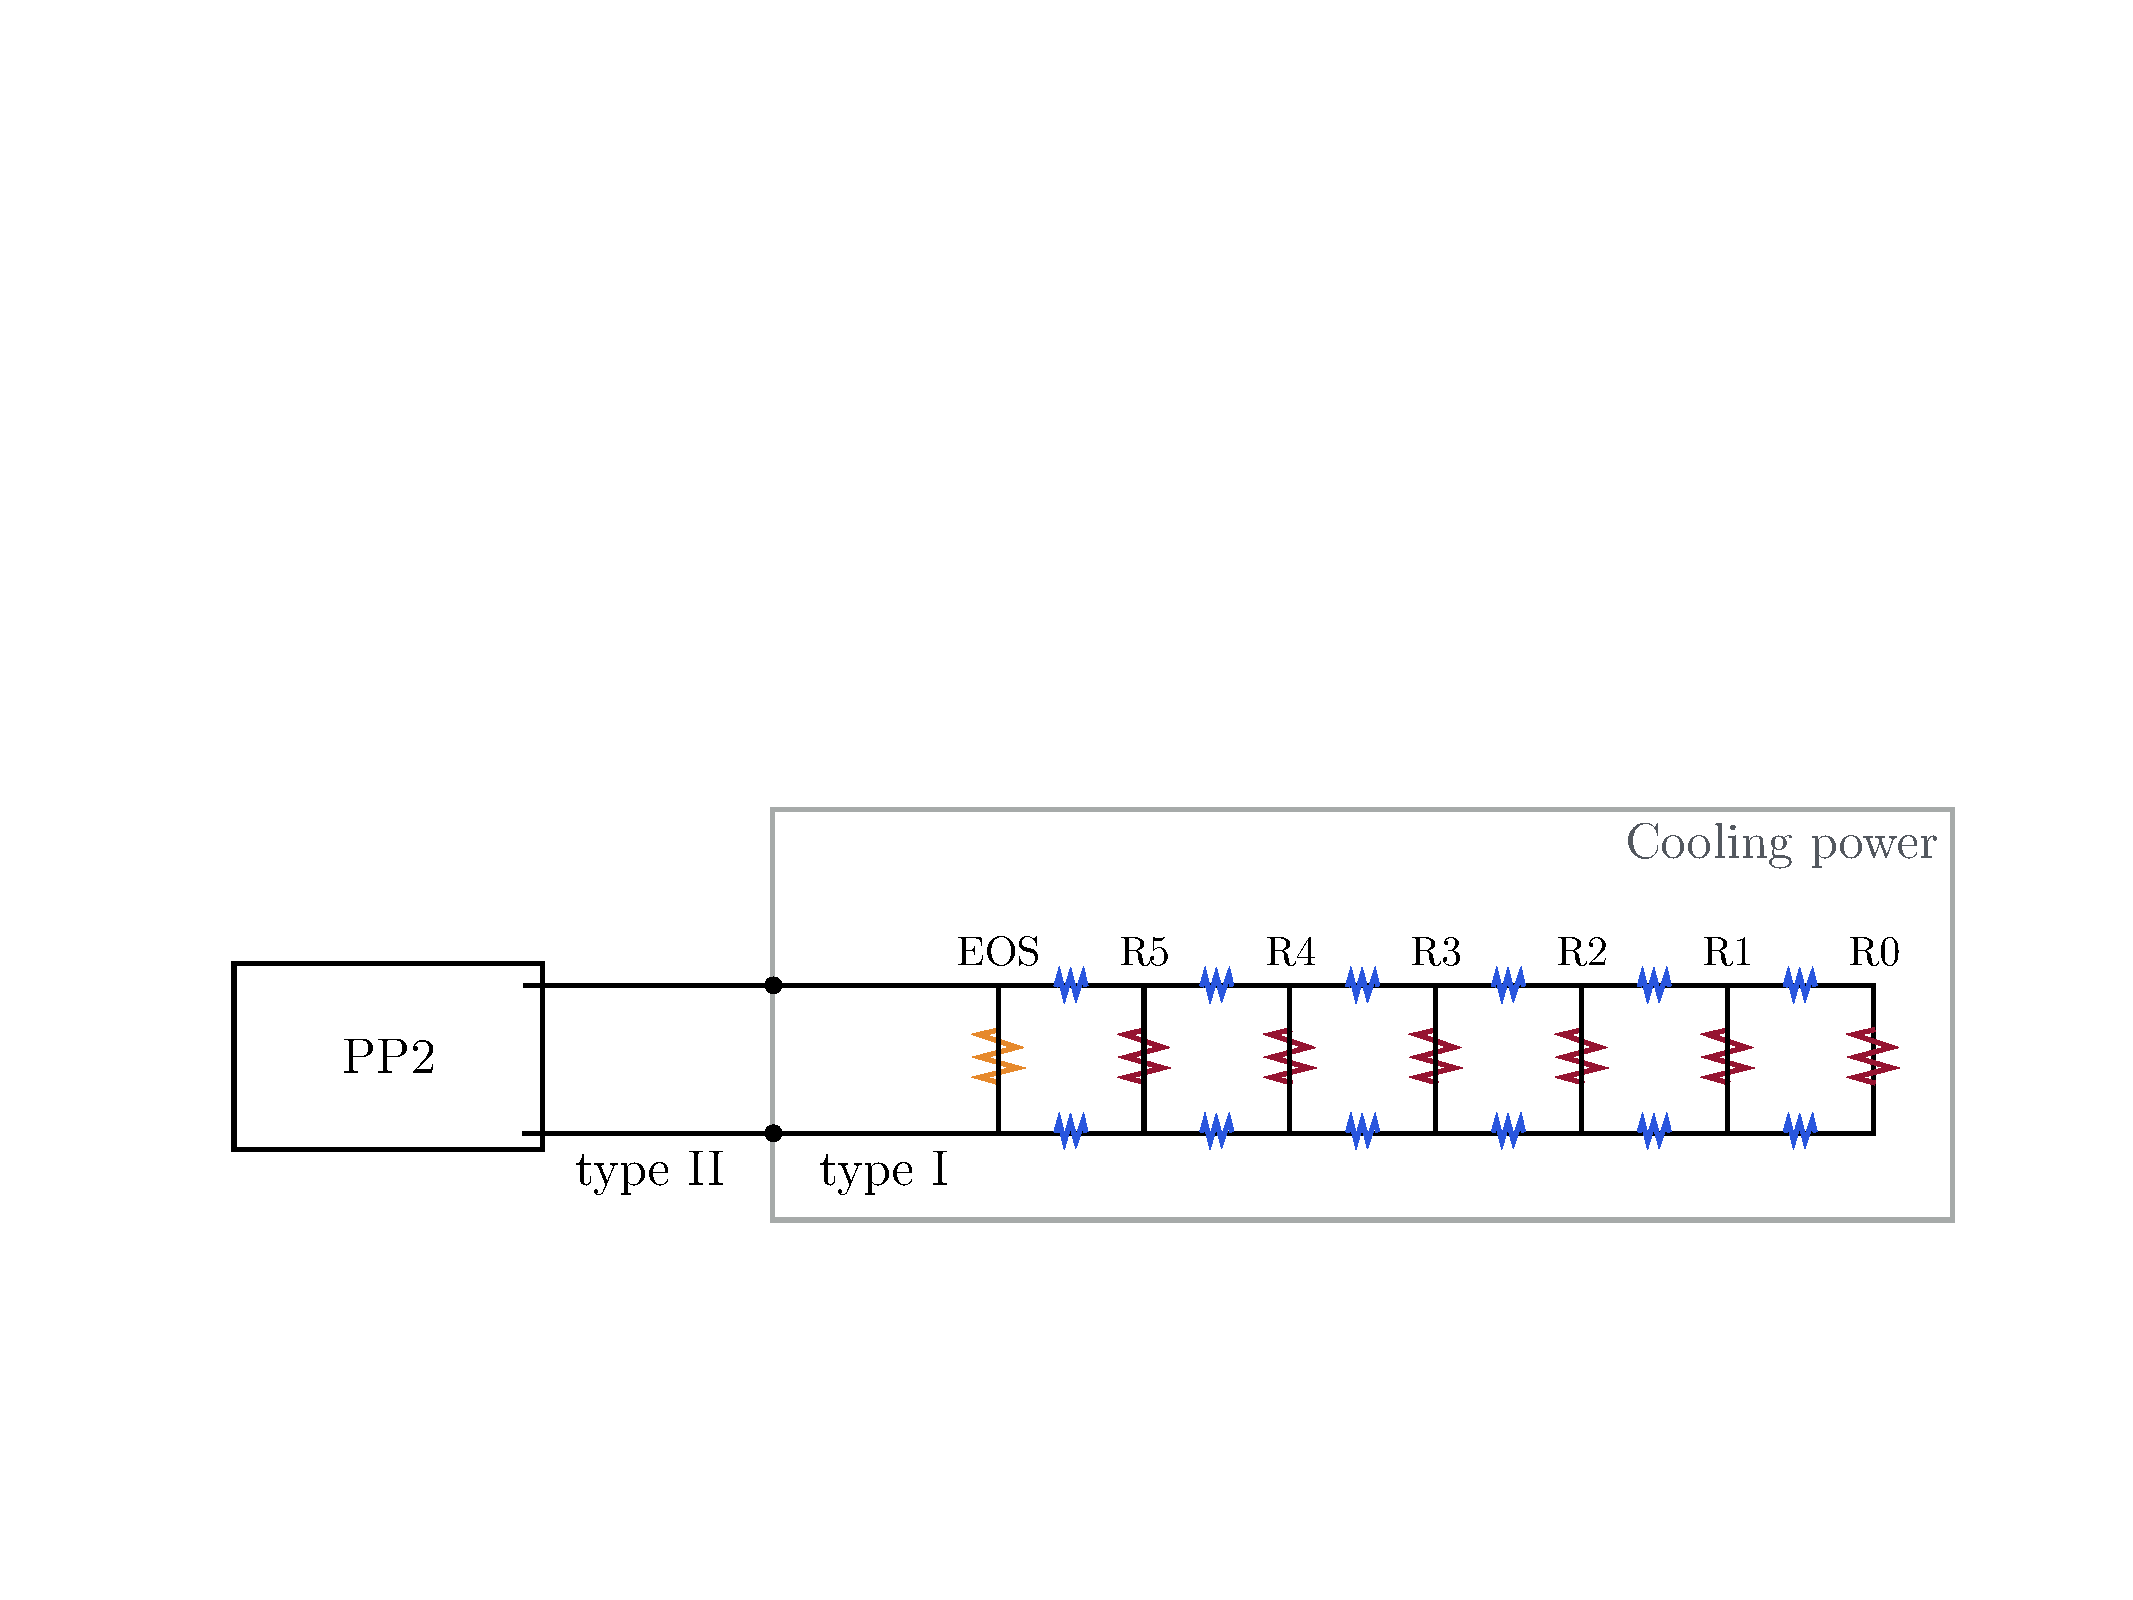
\includegraphics[width=0.74\linewidth]{figures/LV_cartoon.pdf}
\end{center}
\caption{Simplified depcition of the petal LV circuit. The EOS effective resistance is in orange;
the voltage drop from BPOL12V and linPOL12V is in red; the tape resistance is blue.
The type-I cables are counted in the cooling power.}
\label{lv_circuit}
\end{figure}

Figure~\ref{lv_circuit} depicts a simplified version of the LV circuit.

%% The low-voltage is modeled as losing 1V over the length of the petal, with 11V at the EOS and
%% dropping to 10V in R1\footnote{Estimates provided by Pepe Bernabeu.} at beginning-of-life.
%% To ensure consistency between
%% the tape resistance and the voltage drop in the front-end components in each module, (and because I
%% don't have good numbers for endcap tape resistances), tape resistance values are chosen to cause a
%% 1/6~V drop between modules.


The low-voltage will be sensed at the EOS at 11 V, and expected to drop up to 1 V through the length of
the tape, depending on the tape resistance. Estimates of the tape resistance are under investigation;
for now a worst-case tape resistance of 20 m$\Omega$ is used in the endcap.

To ensure consistency between
the tape resistance and the voltage drop in the front-end components in each module,
the voltage drop in the R0 front-end is strategically chosen such that the $\Delta V$
of the R0 front-end plus the total tape $\Delta V$ equals 11 V at the EOS.
The procedure is as follows:
to correctly model the tape current and LV voltage in each module, the model performs its predictions
of each module starting from R0, followed by R1, R2, ... R5. The voltage drop across the front-end
components in R0 is set at 10.79~V. The current in the R0 tape is:
%
\[
I^{R0}_\text{tape} = \frac{P^{R0}_{LV}}{V^{R0}_{LV}}.
\]
When calculating the next-highest module (e.g. R1), the FE voltage is set to the voltage drop of the
previous FE, plus the additional voltage drop due to the tape in the previous module:
\[
V^{Rn}_{LV} = V^{R(n-1)}_{LV} + I^{R(n-1)}_\text{tape} R^{R(n-1)}_\text{tape}.
\]
Likewise, the tape current in module $Rn$ is equal to the current from the module's FE plus the
accumulated current from the previous modules:
\[
I^{Rn}_\text{tape} = \frac{P^{Rn}_{LV}}{V^{Rn}_{LV}} + I^{R(n-1)}_\text{tape}.
\]
With $\Delta V$ at R0 set at 10.79~V, the voltage at the EOS is 11~V in beginning-of-life conditions
(without safety factors).
Note that this calculation occurs at each time step in the model, so power increases due to the TID
bump affect both the FE voltages and the tape current.
(The effect of the bump is less than 0.1~V at the TID bump maximum.)

Table~\ref{voltage_drops} specifies the voltage input at each module given the
chosen tape resistance value of 20~m$\Omega$.

\begin{table}[ht]
\begin{center}
\adjustbox{max width=\textwidth}{ %% just before tabular
\begin{tabular}{|l|l|r|r|r|r|r|r|l|} \hline % data_below
Quantity & Description           &     R0 &     R1 &     R2 &     R3 &     R4 &     R5 & Unit   \\ \hline
\multirow{2}{*}{$V_{in}$} & Input voltage to the BPOL12V &  \multirow{2}{*}{10.79} &  \multirow{2}{*}{10.80} &  \multirow{2}{*}{10.82}
&  \multirow{2}{*}{10.85} &  \multirow{2}{*}{10.89} &  \multirow{2}{*}{10.94} & \multirow{2}{*}{V}      \\
 & and linPOL12V on each module & & & & & & & \\ \hline
$R_\text{tape}$           & Tape resistance in each module &  \multicolumn{6}{c|}{20} & m$\Omega$ \\
\hline\end{tabular}
} %% resize box after tabular
\end{center}
\caption{Voltage inputs for each endcap module. The EOS is assumed to have an 11V input voltage.}
\label{voltage_drops}
\end{table}

\subsection{Low voltage cables}

The low-voltage power calculations follow Georg's treatment, with the exception of the
calculations of module voltages described above.
Several quantities are quoted in the main summary tables:
following Figure~\ref{lv_circuit}, the
quantity ``LV round-trip $\Delta V$ from PP2'' consists of voltage drops from type I and II cables
only, and ``Max LV $V_\text{out}$ at PP2'' represents the voltage drop of the tape plus FE
($\Delta V_{R0} + \Delta V_\text{tape}$), plus the voltage drop of the type I and II cables.

\subsection{High voltage}

% https://edms.cern.ch/ui/file/1889475/10/Bus_Tapes_specs_v10_300118.pdf
%% There will be 4 separate HV lines for barrel and petals. For the petals, the
%% separate HV lines will serve modules: R5, R4, R3 and R2, and R1 and R0. For the
%% barrels, the HV lines will serve modules: 0 to 3, 4 to 7, 8 to 10 and 11 to 13, where
%% module 0 is defined to be the module closest to the centre of the detector and module 13
%% is adjacent to the EoS.

\begin{figure}[ht!]
\begin{center}
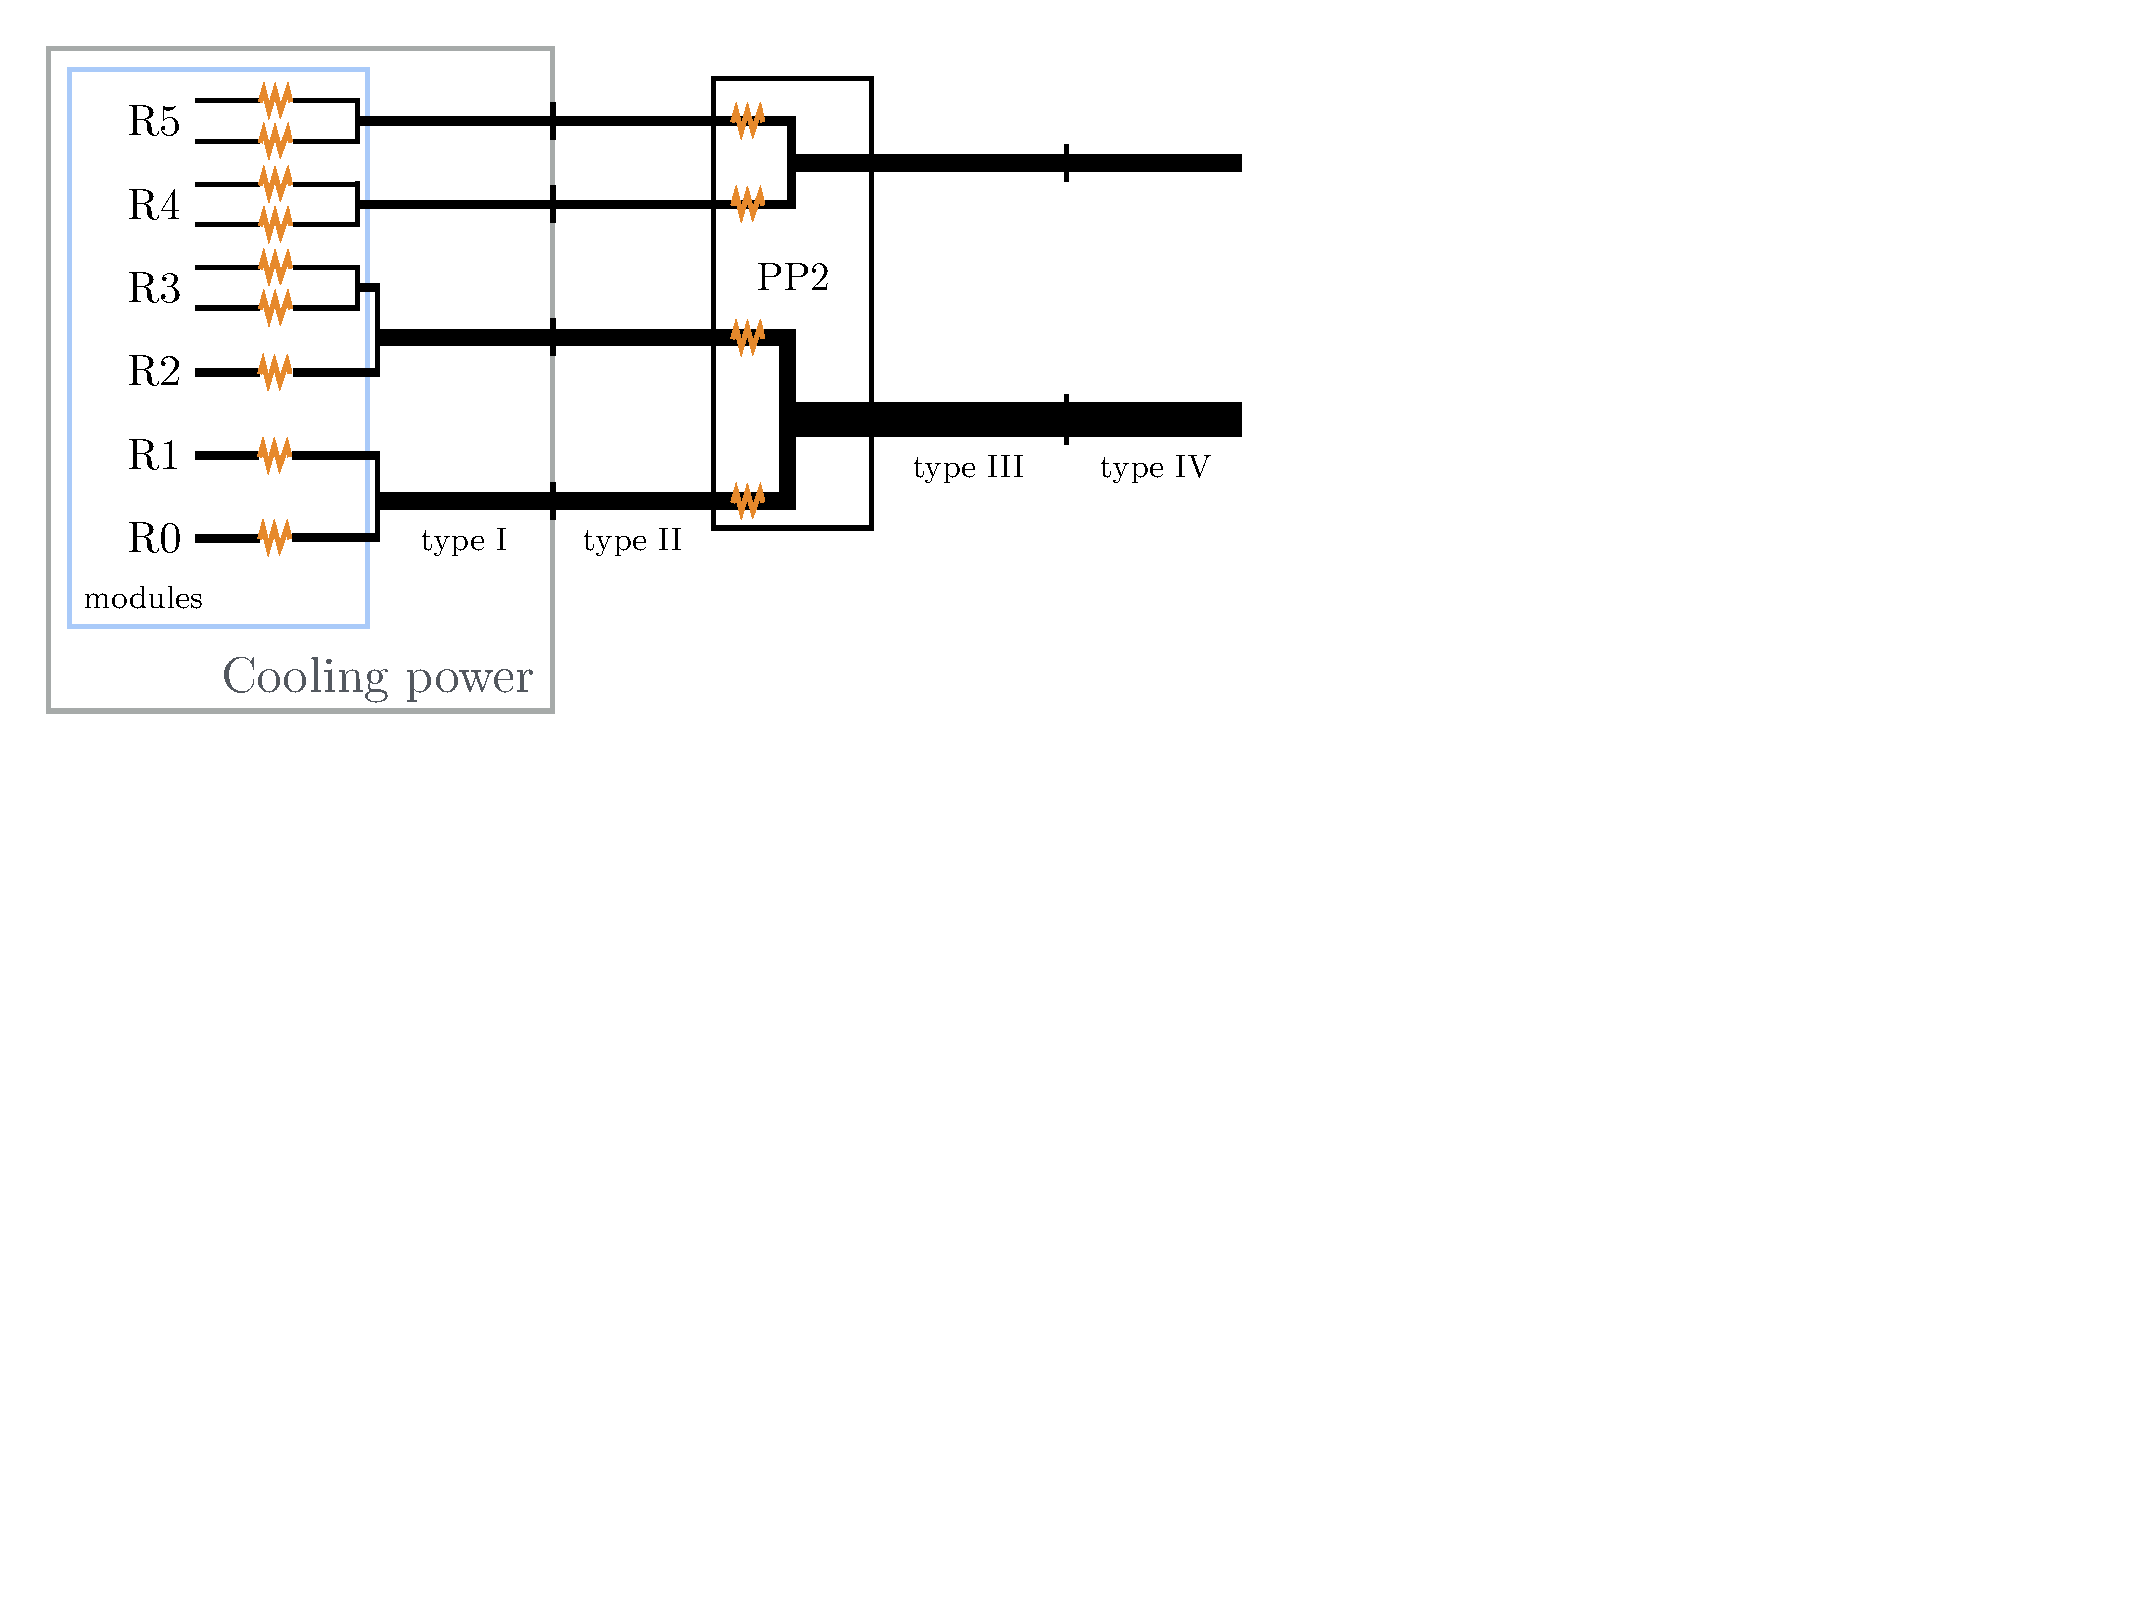
\includegraphics[width=0.60\linewidth]{figures/HV_cartoon.pdf}
\end{center}
\caption{Simplified depcition of the petal HV circuit, showing the HV cable multiplexing scheme. HV filters are shown
in orange. The type-I cables are counted in the cooling power. The HV return current will use the LV return line.}
\label{hv_circuit}
\end{figure}

Figure~\ref{hv_circuit} depicts a simplified version of the HV circuit. Most of the treatment of the
HV voltage and power calculations use the same strategies and equations described in Georg's text, with
the exceptions described below.
{ \bf Important note: the endcap HV tape resistance is currently set to 0. } The expected impact on petal
and total power results is very small.

\def\rhvmuxI{R^\text{HV,cables}_\text{muxI/II}}
\def\rhvmuxIII{R^\text{HV,cables}_\text{muxIII/IV}}

There are four Type I and II HV lines per petal side, which serve modules in the following multiplexing
scheme: (R0 + R1), (R2 + R3), R4, R5\footnote{ See
https://edms.cern.ch/ui/file/1889475/10/Bus\_Tapes\_specs\_v10\_300118.pdf
}. The HV tape and PP2 HV filters are also assumed to be multiplexed in this way. Thus, we can define
a quantity $\rhvmuxI$ to refer to the sum of these resistances:
%
\def\rtape{R^\text{HV}_\text{tape}}
\def\rtypeI{R^\text{HV}_\text{typeI}}
\def\rtypeII{R^\text{HV}_\text{typeII}}
\def\rtypeIII{R^\text{HV}_\text{typeIII}}
\def\rtypeIV{R^\text{HV}_\text{typeIV}}
\[
\rhvmuxI = \rtape + \rtypeI + \rtypeII + R^\text{HV}_\text{PP2}
\]

The multiplexing of the Type III and IV cables is currently
assumed to be (R0 + R1 + R2 + R3) and (R4 + R5). We can define an effective resistance for these
too:
\[
\rhvmuxIII = \rtypeIII + \rtypeIV
\]

Then the HV voltage drops of the services (including the filters on the module) are then:
\def\dvservices{\Delta V^\text{services}}
\begin{align}
\dvservices_\text{HV,R0} =& I^{R0}_S \cdot R_{HV}           + \left(\sum_{X=0,1} I^\text{RX}_S\right) \cdot \rhvmuxI + \left(\sum^3_{X=0} I^\text{RX}_S\right) \cdot \rhvmuxIII \\
\dvservices_\text{HV,R1} =& I^{R1}_S \cdot R_{HV}           + \left(\sum_{X=0,1} I^\text{RX}_S\right) \cdot \rhvmuxI + \left(\sum^3_{X=0} I^\text{RX}_S\right) \cdot \rhvmuxIII \\
\dvservices_\text{HV,R2} =& I^{R2}_S \cdot R_{HV}           + \left(\sum_{X=2,3} I^\text{RX}_S\right) \cdot \rhvmuxI + \left(\sum^3_{X=0} I^\text{RX}_S\right) \cdot \rhvmuxIII \\
\dvservices_\text{HV,R3} =& I^{R3}_S \cdot \frac{R_{HV}}{2} + \left(\sum_{X=2,3} I^\text{RX}_S\right) \cdot \rhvmuxI + \left(\sum^3_{X=0} I^\text{RX}_S\right) \cdot \rhvmuxIII \\
\dvservices_\text{HV,R4} =&                                I^{R4}_S \cdot \left(\frac{R_{HV}}{2} +\rhvmuxI \right)   + \left(\sum_{X=4,5} I^\text{RX}_S\right) \cdot \rhvmuxIII \\
\dvservices_\text{HV,R5} =&                                I^{R5}_S \cdot \left(\frac{R_{HV}}{2} +\rhvmuxI \right)   + \left(\sum_{X=4,5} I^\text{RX}_S\right) \cdot \rhvmuxIII
\end{align}
%
where the contribution from the on-module HV filter is halved in R3, R4 and R5 because of the
two-filter, split-current scheme in those modules.

The HV power dissipated in the HV services, excluding the on-module HV filters (whose power is counted
as part of the module), is:
\def\phvservices{P^\text{services}_\text{HV}}
\[
\phvservices = \rhvmuxI \cdot \left[ \left(\sum_{X=0,1} I^\text{RX}_S\right)^2
                                    +\left(\sum_{X=2,3} I^\text{RX}_S\right)^2
                                    +\left(I^{R4}_S\right)^2
                                    +\left(I^{R5}_S\right)^2
                                    \right]
               + \rhvmuxIII \cdot \left[ \left(\sum^3_{X=0} I^\text{RX}_S\right)^2
                                        +\left(\sum_{X=4,5} I^\text{RX}_S\right)^2
                                        \right]
\]

Table~\ref{cableHVInputs} describes the cable inputs used for the HV power losses.
Note that the HV return current will use the LV return line, meaning the cable one-way
length is not doubled in the HV case when calculating $\Delta V_\text{HV}$ and $\phvservices$.

\begin{table}[ht]
\begin{center}
\adjustbox{max width=\textwidth}{ %% just before tabular
\begin{tabular}{|l|l|r|l|} \hline % data_below
Configurable Item         & Description                          &      Value & Unit        \\ \hline
HVType1ResistancePerMeter & Type 1 HV cable resistance per meter &      0.213 & $\Omega$/m  \\
HVType2ResistancePerMeter & Type 2 HV cable resistance per meter &      0.213 & $\Omega$/m  \\
HVType3ResistancePerMeter & Type 3 HV cable resistance per meter &      0.139 & $\Omega$/m  \\
HVType4ResistancePerMeter & Type 4 HV cable resistance per meter &    0.14286 & $\Omega$/m  \\
LVType1ResistancePerMeter & Type 1 LV cable resistance per meter &      0.021 & $\Omega$/m  \\
LVType2ResistancePerMeter & Type 2 LV cable resistance per meter &     0.0148 & $\Omega$/m  \\
LVType3ResistancePerMeter & Type 3 LV cable resistance per meter &     0.0095 & $\Omega$/m  \\
LVType4ResistancePerMeter & Type 4 LV cable resistance per meter &    0.00127 & $\Omega$/m  \\
PP2Efficiency             & PP2 Efficiency                       &       0.85 &             \\
PP2HVFilterResistance     & PP2 Efficiency                       &      100.0 & $\Omega$    \\
PP2InputVoltage           & PP2 input voltage                    &       48.0 & V           \\
PowerSuppliesEfficency    & Power supplies efficiency            &        0.8 &             \\
Type1LengthOneWay         & Type 1 LV/HV cable one-way length    &       2.44 & m           \\
Type2LengthOneWay         & Type 2 LV/HV cable one-way length    &       15.0 & m           \\
Type3LengthOneWay         & Type 3 LV/HV cable one-way length    &       32.0 & m           \\
Type4LengthOneWay         & Type 4 LV/HV cable one-way length    &       70.0 & m           \\
HV tape resistance        & HV tape resistance                   &        0.0 & $\Omega$    \\
\hline\end{tabular}
} %% resize box after tabular
\end{center}
\caption{HV cable inputs for the endcap}
\label{cableHVInputs}
\end{table}

\clearpage

\section{Other inputs}

\subsection{Total Ionizing Dose and Flux}

In the petal model, the total ionizing dose and fluence are given in Tables~\ref{tid} and~\ref{flux},
respectively. They are taken from ``step 1.9'' results found in the following location\footnote{
Note that a more recent calculation, ``Step 1.9 with Run-2 beam pipe'' or S1.9+R2BP, is not used here.
}:

\url{https://twiki.cern.ch/twiki/bin/view/Atlas/RadiationBackgroundSimulationsFullyInclinedAt4#Step_1_9}

\begin{table}[ht]
\begin{centering}\adjustbox{max width=\textwidth}{ %% just before tabular
\begin{tabular}{|l|r|r|r|r|r|r|r|} \hline % data_below
  & & \multicolumn{6}{c|}{Disk} \\
\multirow{6}{*}{Ring}
 &   &       0 &       1 &       2 &       3 &       4 &       5 \\ \hline
 & 5 &    4700 &    5000 &    5300 &    5800 &    6400 &    7000 \\ 
 & 4 &    6200 &    6700 &    6700 &    7200 &    7900 &    8900 \\ 
 & 3 &    9000 &    9200 &    9500 &   10500 &   10800 &   12100 \\ 
 & 2 &   11000 &   11300 &   11400 &   12100 &   12800 &   14300 \\ 
 & 1 &   14400 &   14800 &   15500 &   16500 &   18100 &   20100 \\ 
 & 0 &   22700 &   23900 &   24800 &   26800 &   29100 &   31100 \\ 
\hline\end{tabular}
} %% resize box after tabular
\caption{TID in 3000 fb$^{-1}$ of collected data [Rad]}
\label{tid}
\end{centering}
\end{table}


\begin{table}[ht]
\begin{centering}\adjustbox{max width=\textwidth}{ %% just before tabular
\begin{tabular}{|l|r|r|r|r|r|r|r|} \hline % data_below
  & & \multicolumn{6}{c|}{Disk} \\
\multirow{6}{*}{Ring}
 &   &        0 &        1 &        2 &        3 &        4 &        5 \\ \hline
 & 5 & 2.26e+14 & 2.36e+14 & 2.56e+14 & 2.84e+14 & 3.21e+14 & 3.77e+14 \\ 
 & 4 & 2.53e+14 & 2.65e+14 & 2.85e+14 & 3.12e+14 & 3.56e+14 & 4.25e+14 \\ 
 & 3 & 3.01e+14 & 3.11e+14 & 3.32e+14 & 3.66e+14 & 4.11e+14 & 5.00e+14 \\ 
 & 2 & 3.31e+14 & 3.41e+14 & 3.62e+14 & 3.95e+14 & 4.47e+14 & 5.47e+14 \\ 
 & 1 & 3.93e+14 & 4.03e+14 & 4.22e+14 & 4.57e+14 & 5.14e+14 & 6.36e+14 \\ 
 & 0 & 5.03e+14 & 5.12e+14 & 5.38e+14 & 5.67e+14 & 6.25e+14 & 7.74e+14 \\ 
\hline\end{tabular}
} %% resize box after tabular
\caption{Total flux in 3000 fb$^{-1}$ of collected data [$n_\text{eq}/$cm$^2$]}
\label{flux}
\end{centering}
\end{table}

\subsection{Full list of inputs}

A full list of model inputs, output from the code, is listed below. The safety factors shown here
describe the worst-case safety factor scenario.

\begin{table}[ht]
\begin{centering}\adjustbox{max width=\textwidth}{ %% just before tabular
\begin{tabular}{|l|l|r|l|} \hline % data_below
Configurable Item                    & Description                                                  &      Value & Unit        \\ \hline
AbcTidBump.ModelVersion              & TID parameterization Model Version                           &        v02 & --          \\ 
CableLosses.lossouter                & Cable losses from PP1 to USA15                               &       0.05 & --          \\ 
CableLosses.losstype1                & Cable losses from service modules                            &       0.05 & --          \\ 
EOSComponents.Veos                   & EOS input voltage                                            &       11.0 & V           \\ 
EOSComponents.gbld12I                & Current in GBLD10 1.2V circuit                               &     0.0095 & A           \\ 
EOSComponents.gbld25I                & Current in GBLD10 2.5V circuit                               &      0.018 & A           \\ 
EOSComponents.gbtiaI                 & Current in GBTIA (voltage is 2.5 V)                          &      0.053 & A           \\ 
EOSComponents.lpgbtI                 & Current in lpGBT (voltage is 1.2 V)                          &      0.625 & A           \\ 
FrontEndComponents.abcIa             & ABC analog current                                           &       0.07 & A           \\ 
FrontEndComponents.abcId             & ABC digital current                                          &     0.0425 & A           \\ 
FrontEndComponents.amac15I           & AMAC current of 1.5V circuit                                 &     0.0517 & A           \\ 
FrontEndComponents.amac3I            & AMAC current of 3V circuit                                   &     0.0012 & A           \\ 
FrontEndComponents.hccIa             & HCC analog current                                           &      0.075 & A           \\ 
FrontEndComponents.hccId             & HCC digital current                                          &      0.125 & A           \\ 
FrontEndComponents.hybridV           & Hybrid voltage                                               &        1.5 & V           \\ 
FrontEndComponents.ldoI              & LDO quiescent current                                        &     0.0019 & A           \\ 
Layout.Detector                      & barrel or endcap geometry                                    &     Endcap & --          \\ 
Layout.npetals                       & Number of petals per ring                                    &         32 & --          \\ 
NominalPower.Rtape                   & tape resistance is 0.01 $\Omega$ per module worst case       &       0.01 & $\Omega$    \\ 
PoweringEfficiency.DCDC2eff          & Efficiency of EOS DCDC2 converter                            &       0.88 & --          \\ 
PoweringEfficiency.ModelVersion      & Feast Efficiency Model Version                               &        v01 & --          \\ 
SafetyFactors.TIDpessimistic         & TID is pessimistic parameterization?                         &       True & --          \\ 
SafetyFactors.safetycurrenta         & Fractional analog current safety factor increase             &       0.05 & --          \\ 
SafetyFactors.safetycurrentd         & Fractional digital current safety factor increase            &        0.2 & --          \\ 
SafetyFactors.safetyfluence          & Fractional safety factor increase over 3935 fb$^{-1}$        &        0.5 & --          \\ 
SafetyFactors.safetythermalimpedance & Fractional thermal impedance safety factor increase          &        0.2 & --          \\ 
SafetyFactors.vbias                  & HV bias voltage (default is 500V)                            &      700.0 & V           \\ 
SensorProperties.Rhv                 & HV resistors are 2 times 5k                                  &    10000.0 & $\Omega$    \\ 
SensorProperties.Rhvmux              & parallel resistor for MUX operation is 10M                   & 10000000.0 & $\Omega$    \\ 
StripsThermalModel.GitHash           & Git hash (for internal use)                                  &    c50c7a4 & --          \\ 
ThermalImpedances.reos               & Thermal impedance of EOS                                     &       15.0 & K/W         \\ 
ThermalImpedances.rs                 & Thermal impedance of Sensor                                  &       0.02 & K/W         \\ 
cooling                              & Coolant temperature scenario (usually flat, or ramping down) &    flat-35 & $^{\circ}$C \\ 
\hline\end{tabular}
} %% resize box after tabular
\end{centering}
\caption{Model inputs common to all endcap modules.}
\end{table}

\begin{table}[ht]
\begin{centering}\adjustbox{max width=\textwidth}{ %% just before tabular
\begin{tabular}{|l|l|r|r|r|r|r|r|l|} \hline % data_below
Configurable Item         & Description                                    &     R0 &     R1 &     R2 &     R3 &     R4 &     R5 & Unit   \\ \hline
NominalPower.Hybrid0.nabc & --                                             &      8 &     10 &     12 &      7 &      8 &      9 & --     \\ 
NominalPower.Hybrid1.nabc & --                                             &      9 &     11 &      0 &      7 &      8 &      9 & --     \\ 
NominalPower.Hybrid2.nabc & --                                             &      0 &      0 &      0 &      7 &      0 &      0 & --     \\ 
NominalPower.Hybrid3.nabc & --                                             &      0 &      0 &      0 &      7 &      0 &      0 & --     \\ 
NominalPower.Hybrid0.nhcc & --                                             &      1 &      1 &      2 &      0 &      0 &      0 & --     \\ 
NominalPower.Hybrid1.nhcc & --                                             &      1 &      1 &      0 &      2 &      2 &      2 & --     \\ 
NominalPower.Hybrid2.nhcc & --                                             &      0 &      0 &      0 &      0 &      0 &      0 & --     \\
NominalPower.Hybrid3.nhcc & --                                             &      0 &      0 &      0 &      2 &      0 &      0 & --     \\ 
NominalPower.nabc         & Number of ABCs on the hybrid                   &     17 &     21 &     12 &     28 &     16 &     18 & --     \\ 
NominalPower.namac        & Number of AMACs on the hybrid                  &      1 &      1 &      1 &      2 &      1 &      1 & --     \\ 
NominalPower.nfeast       & Number of FEAST chips on the hybrid            &      1 &      1 &      1 &      2 &      1 &      1 & --     \\ 
NominalPower.ngbld        & Number of GBLDs on this module's EOS           &      0 &      0 &      0 &      0 &      0 &      1 & --     \\ 
NominalPower.ngbtia       & Number of GBTIAs on this module's EOS          &      0 &      0 &      0 &      0 &      0 &      1 & --     \\ 
NominalPower.nhcc         & Number of HCCs on the hybrid                   &      2 &      2 &      2 &      4 &      2 &      2 & --     \\ 
NominalPower.nlpgbt       & Number of lpGBTs on this module's EOS          &      0 &      0 &      0 &      0 &      0 &      1 & --     \\ 
PoweringEfficiency.Vfeast & Feast input voltage                            &  10.00 &  10.17 &  10.33 &  10.50 &  10.67 &  10.83 & V      \\ 
SensorProperties.area     & Sensor area on the module                      &   92.0 &   91.0 &   76.0 &  164.0 &  178.0 &  186.0 & cm$^2$ \\ 
ThermalImpedances.rabc    & Thermal impedance of ABCs                      &  0.927 &  0.661 &  1.529 &  0.582 &  1.316 &  1.151 & K/W    \\ 
ThermalImpedances.rc      & Thermal impedance of Module+EOS common pathway &  0.000 &  0.000 &  0.000 &  0.000 &  0.000 &  0.091 & K/W    \\ 
ThermalImpedances.rfeast  & Thermal impedance of FEAST(s)                  & 16.627 & 17.936 & 18.282 & 11.361 & 17.847 & 16.470 & K/W    \\ 
ThermalImpedances.rhcc    & Thermal impedance of HCCs                      & 12.485 & 12.719 & 13.833 &  6.808 & 12.669 & 12.905 & K/W    \\ 
ThermalImpedances.rm      & Thermal impedance of module pathway            &  0.793 &  1.004 &  1.432 &  0.859 &  0.873 &  0.486 & K/W    \\ 
\hline\end{tabular}
} %% resize box after tabular
\end{centering}
\caption{Model inputs specific to endcap module type (R0, R1, etc.).}
\end{table}

\clearpage

\newcommand{\mry}[2]{
\multirow{#1}{*}{Year #2}
}

\section{Results}

\subsection{Description of Output}
\subsubsection{Module-level quantities}
%% \let\itemsepa\itemsep
%% \renewcommand\itemsep{1.0}
Avearage temperatures are reported on each module for each of the following: sensor, ABC, HCC, Feast,
and EOS.

Reported power values for each module: 
\begin{itemize}
\setlength\itemsep{0.0em}
\item Sensor Q (one side)
\item EOS power (one side)
\item LV tape power loss due to items on module (one side)
\item Cumulative LV tape power loss (one module one side):
Power loss in the tape associated to this module, due to the current from items on the module, plus
current from previous modules.
\item HV power serial resistors (one side)
\item HV power parallel resistor (one side)
\item Total HV power (including leakage) (one side)
\item Module power (one side) (no EOS): front-end + HV + tape
\end{itemize}

Reported current values for each module:
\begin{itemize}
\setlength\itemsep{0.0em}
\item Sensor (leakage) current (one module side)
\item LV tape current (one side) due to items on module
\item LV tape current (one side)
\item Tape current load due to EOS (one side)
\item ABC and HCC digital current
\item Hybrid 0 (1,2,3) current (if applicable)
\item FEAST current (load per Feasts, in case there is more than one Feast)
\item FEAST current (input, both Feasts, in case there is more than one Feast.)
\end{itemize}

Other reported module-level values:
\begin{itemize}
\setlength\itemsep{0.0em}
\item Feast efficiency
\item Sensor Q headroom factor
\item Coolant temperature headroom
\end{itemize}
%% \let\itemsep\itemsepa

\subsubsection{Petal-level quantities}

The following items are reported for petals at each disk position:
\begin{itemize}
\setlength\itemsep{0.0em}
\item Total power in petal located at Disk $n$ (including the EOS) (one petal side)
\item Total sensor Q in petal located at Disk $n$ (one side)
\item HV power in petal located at Disk $n$ (one side)
\item LV tape current in petal located at Disk $n$ (including the EOS) (one side)
\item Total sensor (leakage) current in petal located at Disk $n$ (one side)
\end{itemize}

\subsubsection{Full system quantities}

\begin{itemize}
\setlength\itemsep{0.0em}
\item Total power in both endcaps, including cable losses -- modeled as 
5\%$\times$5\% for cable losses from the service modules and cable losses from PP1 to USA15 (10.25\% total loss).
More realistic cable losses are under construction.
\item Total HV power (sensor + resistors) in both endcaps
\end{itemize}

\subsection{Nominal and Pessimistic scenarios}

Table~\ref{results_summary} shows the power estimates, properties (temperature) of the sensor and
FEAST, as well as HV and LV currents. Two scenarios are shown: one in which no safety factors are
applied, and one in which all safety factors (Fluence, thermal impedance, digital and analog current,
TID parameterization, and HV bias) are applied. In both cases, a wide range of cooling scenarios
(from $-35^\circ$C to $-35^\circ$C coolant temperature) are shown, as well as the ``ramp'' scenario
in which the temperature is ramped down from $0^\circ$C to $-35^\circ$C over the course of 9 years
(the same as used in the barrel).

In the nominal scenario, the Endcap System has a total power (including cable losses) between 32.1
and 38.3 kW (it varies due to the effect of the TID bump in the electronics).
In the worst-case safety factor scenario, the total power is 36.8-46.7 kW.

In places where thermal runaway occurs, the R3 module reaches thermal runaway before the others
(although at higher temperatures in the pessimistic safety-factor scenario, all endcap modules
eventually run away).

It is also important to note that runaway always occurs near the end of the detector life, rather than
at the TID bump.

\let\arraystretcha\arraystretch
\renewcommand\arraystretch{1.15} % 1.6

\begin{table}[ht]
\begin{subtable}[t]{.99\linewidth}
\begin{centering}\adjustbox{max width=\textwidth}{ %% just before tabular
\begin{tabular}{|l|l|r|r|r|r|r|r|} \hline % data_below
\multirow{5}{*}{Safety Factors} & Fluence                                        &           0.0 &           0.0 &           0.0 &           0.0 &           0.0 &           0.0 \\ 
                                & $R_{T}$                                        &           0.0 &           0.0 &           0.0 &           0.0 &           0.0 &           0.0 \\ 
                                & $I_D$                                          &           0.0 &           0.0 &           0.0 &           0.0 &           0.0 &           0.0 \\ 
                                & $I_A$                                          &           0.0 &           0.0 &           0.0 &           0.0 &           0.0 &           0.0 \\ 
                                & TID parameterization                           &       nominal &       nominal &       nominal &       nominal &       nominal &       nominal \\ \hline
\multirow{2}{*}{HV, Cooling}    & Voltage [V]                                    &         500.0 &         500.0 &         500.0 &         500.0 &         500.0 &         500.0 \\ 
                                & Cooling [$^\circ$C]                            &    flat $-$35 &    flat $-$30 &    flat $-$25 &    flat $-$20 &    flat $-$15 &    ramp $-$35 \\ \hline
\multirow{3}{*}{Endcap System}  & Minimum power [kW]                             &          32.1 &          32.2 &          32.3 &          32.4 &   \bf Runaway &          32.9 \\ 
                                & Maximum power [kW]                             &          38.3 &          37.3 &          36.6 &          40.3 &   \bf Year 11 &          36.2 \\ 
                                & Maximum $P_\text{HV}$ [kW]                     &          1.08 &          1.96 &          3.65 &          7.22 &      \bf (R3) &          2.10 \\ \hline
\multirow{2}{*}{Petal-level}    & Max petal LV $I_\text{tape}$ load [A]          &          4.32 &          4.20 &          4.11 &          4.03 &   \mry{2}{11} &          3.93 \\ 
                                & Max petal power [W]                            &          45.8 &          44.6 &          44.7 &          52.5 &               &          43.7 \\ \hline
R0                              & \multirow{6}{*}{Min/Max Power [W]}             &   5.31 / 8.01 &   5.33 / 7.56 &   5.35 / 7.20 &   5.37 / 7.26 &   \mry{6}{11} &   5.39 / 6.43 \\ 
R1                              &                                                &   6.36 / 8.75 &   6.38 / 8.36 &   6.41 / 8.05 &   6.44 / 8.56 &               &   6.46 / 7.53 \\ 
R2                              &                                                &   4.19 / 5.23 &   4.20 / 5.07 &   4.21 / 4.95 &   4.23 / 5.64 &               &   4.27 / 4.86 \\ 
R3                              &                                                &   9.36 / 11.6 &   9.39 / 11.3 &   9.42 / 11.4 &   9.45 / 14.4 &               &   9.57 / 10.9 \\ 
R4                              &                                                &   5.20 / 6.45 &   5.22 / 6.27 &   5.23 / 6.32 &   5.25 / 7.49 &               &   5.33 / 6.21 \\ 
R5                              &                                                &   5.72 / 7.01 &   5.74 / 6.82 &   5.76 / 6.68 &   5.78 / 7.38 &               &   5.87 / 6.71 \\ \hline
\multirow{5}{*}{Components}     & Max $I_{HV}$ per module [mA]                   &    0.965 (R3) &     1.85 (R3) &     3.65 (R3) &     8.40 (R3) &   \mry{5}{11} &     1.95 (R3) \\ 
                                & Max sensor T [$^\circ$C], Y1                   &      -27 (R3) &    -21.9 (R3) &    -16.9 (R3) &    -11.9 (R3) &               &     8.21 (R3) \\ 
                                & Max sensor T [$^\circ$C], Y14                  &    -26.5 (R3) &    -21.1 (R3) &    -15.2 (R3) &    -7.56 (R3) &               &    -26.5 (R3) \\ 
                                & Max sensor T [$^\circ$C], Max                  &      -25 (R3) &    -20.3 (R3) &    -15.2 (R3) &    -7.56 (R3) &               &     8.50 (R3) \\ 
                                & Max $T_\text{Feast}$                           &     28.5 (R1) &     30.3 (R1) &     32.9 (R1) &     36.2 (R1) &               &     49.3 (R1) \\ \hline
\multirow{2}{*}{Headroom}       & Min $Q_{sensor}$ Headroom [$Q_{S,crit}/Q_{S}$] &     7.64 (R3) &     4.27 (R3) &     2.37 (R3) &     1.23 (R3) &   \mry{2}{11} &     4.37 (R3) \\ 
                                & Min Coolant Temp Headroom [$^\circ$C]          &     19.0 (R3) &     13.8 (R3) &     8.35 (R3) &     2.01 (R3) &               &     15.3 (R3) \\ 
\hline\end{tabular}
} %% resize box after tabular
\end{centering}
\caption{Summary of nominal (no safety factors) scenarios, with different coolant temperatures.}
\end{subtable}

\vspace{5mm}

\begin{subtable}[t]{.99\linewidth}
\begin{centering}\adjustbox{max width=\textwidth}{ %% just before tabular
\begin{tabular}{|l|l|r|r|r|r|r|r|} \hline % data_below
\multirow{5}{*}{Safety Factors} & Fluence                                        &           0.5 &          0.5 &           0.5 &           0.5 &           0.5 &           0.5 \\ 
                                & $R_{T}$                                        &           0.2 &          0.2 &           0.2 &           0.2 &           0.2 &           0.2 \\ 
                                & $I_D$                                          &           0.2 &          0.2 &           0.2 &           0.2 &           0.2 &           0.2 \\ 
                                & $I_A$                                          &          0.05 &         0.05 &          0.05 &          0.05 &          0.05 &          0.05 \\ 
                                & TID parameterization                           &   pessimistic &  pessimistic &   pessimistic &   pessimistic &   pessimistic &   pessimistic \\ \hline
\multirow{2}{*}{HV, Cooling}    & Voltage [V]                                    &         700.0 &        700.0 &         700.0 &         700.0 &         700.0 &         700.0 \\ 
                                & Cooling [$^\circ$C]                            &    flat $-$35 &   flat $-$30 &    flat $-$25 &    flat $-$20 &    flat $-$15 &    ramp $-$35 \\ \hline
\multirow{3}{*}{Endcap System}  & Minimum power [kW]                             &          36.8 &         36.9 &   \bf Runaway &   \bf Runaway &   \bf Runaway &          37.8 \\ 
                                & Maximum power [kW]                             &          46.7 &         45.3 &   \bf Year 10 &   \bf Year  7 &   \bf Year  6 &          45.3 \\ 
                                & Maximum $P_\text{HV}$ [kW]                     &          3.10 &         6.28 &   \bf (R3)    &   \bf (all)   &   \bf (all)   &          6.52 \\ \hline
\multirow{2}{*}{Petal-level}    & Max petal LV $I_\text{tape}$ load [A]          &          5.34 &         5.15 &   \mry{2}{10} &    \mry{2}{7} &    \mry{2}{6} &          4.57 \\ 
                                & Max petal power [W]                            &          56.8 &         55.9 &               &               &               &          56.7 \\ \hline
R0                              & \multirow{6}{*}{Min/Max Power [W]}             &   6.07 / 10.6 &  6.09 / 9.95 &   \mry{6}{10} &    \mry{6}{7} &    \mry{6}{6} &   6.24 / 8.01 \\ 
R1                              &                                                &   7.31 / 11.5 &  7.35 / 11.0 &               &               &               &   7.55 / 9.44 \\ 
R2                              &                                                &   4.78 / 6.55 &  4.79 / 6.28 &               &               &               &   4.88 / 6.10 \\ 
R3                              &                                                &   10.7 / 14.1 &  10.7 / 15.8 &               &               &               &   11.0 / 15.7 \\ 
R4                              &                                                &   5.96 / 8.05 &  5.98 / 7.75 &               &               &               &   6.12 / 8.08 \\ 
R5                              &                                                &   6.56 / 8.99 &  6.58 / 8.61 &               &               &               &   6.76 / 8.40 \\ \hline
\multirow{5}{*}{Components}     & Max $I_{HV}$ per module [mA]                   &     2.48 (R3) &    6.51 (R3) &   \mry{5}{10} &    \mry{5}{7} &    \mry{5}{6} &     6.29 (R3) \\ 
                                & Max sensor T [$^\circ$C], Y1                   &      -24 (R3) &   -18.9 (R3) &               &               &               &     11.3 (R3) \\ 
                                & Max sensor T [$^\circ$C], Y14                  &    -22.1 (R3) &   -13.6 (R3) &               &               &               &    -22.1 (R3) \\ 
                                & Max sensor T [$^\circ$C], Max                  &    -20.4 (R3) &   -13.6 (R3) &               &               &               &     12.5 (R3) \\ 
                                & Max $T_\text{Feast}$                           &     75.2 (R1) &    75.3 (R1) &               &               &               &     79.9 (R1) \\ \hline
\multirow{2}{*}{Headroom}       & Min $Q_{sensor}$ Headroom [$Q_{S,crit}/Q_{S}$] &     2.09 (R3) &    1.11 (R3) &   \mry{2}{10} &    \mry{2}{7} &    \mry{2}{6} &     1.16 (R3) \\ 
                                & Min Coolant Temp Headroom [$^\circ$C]          &     6.73 (R3) &   0.943 (R3) &               &               &               &     1.53 (R3) \\ 
\hline\end{tabular}
} %% resize box after tabular
\end{centering}
\caption{Summary of worst-case safety factor scenarios, with different coolant temperatures.}
\end{subtable}
\caption{Comparing nominal and worst-case and safety factor scenarios.}
\label{results_summary}
\end{table}
\let\arraystretch\arraystretcha

\clearpage

\subsection{Interpretation and Main Takeaways}

Two particularly important quantities to monitor are the $Q_{sensor}$ headroom and the coolant
temperature headroom. The $Q_{sensor}$ headroom is the multiplicative factor
$[Q_{s,critical}/Q_{s,current}]$ by which the sensor $Q$ can increase before reaching thermal runaway
(when this value falls to 1, thermal runaway has occurred). The coolant temperature headroom is the
number of degrees C that you could raise the coolant temperature before thermal runaway occurs (the
headroom falls to 0 at thermal runaway). Even without any safety factors, the $Q_{sensor}$ headroom
is below 10; with all of the safety factors applied, the headroom is around 2. The temperature
headroom tells a similar story.

Two questions that can be asked is how to improve the sensor $Q$ headroom, and, since there are many
moving parts in the model, which methods of improving the sensor $Q$ headroom are most effective? The
answer can be addressed by evaluating the effect of each individual safety factor on the sensor $Q$
headroom (and/or the coolant headroom).

Table~\ref{detailed_safety_table} offers a detailed look at the effect of each individual safety
factor; the ``safety factor scenarios'' are ordered according to which scenario has the larger impact
on the minimum sensor $Q$ headroom (minimum sensor $Q$ headroom means the minimum among all of the sensors in
the endcap, at any point in time). According to the results in the table, the thermal impedance
$R_T$ (with a +20\% safety factor) has the largest impact on the sensor $Q$ headroom,
followed by the HV bias (the safety factor is 700 V), and finally the
currents of the ABC, HCC and AMAC\footnote{
The current is typically dominated by the ABC ($\sim$80\%), followed by the HCC ($\sim$20\%). The AMAC
contributes about 1\% to the total power.}.
Note that the fluence safety factor is out of our control, and the nature of the TID bump does not
have any impact on the sensor $Q$ headroom, since its effect is minimal at the detector end-of-life.

The outlook can be ``improved'' in two ways: first, by improving the accuracy of the safety factors.
In other words, if we can e.g. improve the endcap thermal model and build confidence that the thermal
impedance safety factor should be 10\% rather than 20\%, then our worst-case scenarios will have
larger sensor $Q$ headroom values. Another example would be to guarantee that the HV will never run
above 650V. Of course, the margin for error would not have changed---only our confidence that we can
run within that margin of error.

The outlook can also be improved by physical changes to the petal. This includes pipe rerouting, 
using more thermally conductive material, etc. to reduce the thermal impedance of the material
underneath the sensor. It could include making changes to the ABC chip to reduce the current.
These changes would have the effect of reducing the temperature of the sensors, thus increasing the
sensor $Q$ headroom.

\begin{table}[ht]
\begin{centering}\adjustbox{max width=\textwidth,max totalheight=\textheight}{ %% just before tabular
\begin{tabular}{|ccccc|cc|rrrr|r|r|} \hline % data_below
\multicolumn{5}{|c|}{Safety factor} & $V_{bias}$ & Cooling & Endcaps max & Endcaps max & Min sensor $Q$ & Min Coolant\\
Fluence & $R_{T}$ & $I_D$ & $I_A$ &   TID &   [V] & [$^\circ$C] & \multicolumn{1}{l}{power [kW]} & \multicolumn{1}{l}{HV [kW]} & \multicolumn{1}{l}{headroom} & \multicolumn{1}{l|}{headroom [$^\circ$C]} \\ \hline
0.0     &     0.0 &   0.0 &   0.0 & False & 500.0 &  $-$35 flat &      38.3 &    1.08 &      7.64 &       19.0 \\ 
0.5     &     0.0 &   0.0 &   0.0 & False & 500.0 &  $-$35 flat &      39.2 &    1.59 &      5.05 &       14.9 \\ 
0.5     &     0.0 &   0.0 &   0.0 &  True & 500.0 &  $-$35 flat &      41.3 &    1.59 &      5.05 &       14.9 \\ 
0.5     &     0.0 &   0.2 &  0.05 & False & 500.0 &  $-$35 flat &      44.9 &    1.75 &      4.45 &       13.8 \\ 
0.5     &     0.0 &   0.0 &   0.0 & False & 700.0 &  $-$35 flat &      39.4 &    2.32 &      3.60 &       11.6 \\ 
0.5     &     0.2 &   0.0 &   0.0 & False & 500.0 &  $-$35 flat &      38.9 &    1.86 &      3.44 &       11.4 \\ 
0.5     &     0.2 &   0.2 &  0.05 &  True & 700.0 &  $-$35 flat &      46.7 &    3.10 &      2.09 &       6.73 \\ \hline
0.0     &     0.0 &   0.0 &   0.0 & False & 500.0 &  $-$30 flat &      37.3 &    1.96 &      4.27 &       13.8 \\ 
0.5     &     0.0 &   0.0 &   0.0 & False & 500.0 &  $-$30 flat &      38.1 &    2.98 &      2.77 &       9.55 \\ 
0.5     &     0.0 &   0.0 &   0.0 &  True & 500.0 &  $-$30 flat &      39.8 &    2.98 &      2.77 &       9.55 \\ 
0.5     &     0.0 &   0.2 &  0.05 & False & 500.0 &  $-$30 flat &      43.6 &    3.31 &      2.43 &       8.34 \\ 
0.5     &     0.0 &   0.0 &   0.0 & False & 700.0 &  $-$30 flat &      38.3 &    4.37 &      1.97 &       6.29 \\ 
0.5     &     0.2 &   0.0 &   0.0 & False & 500.0 &  $-$30 flat &      37.9 &    3.58 &      1.85 &       5.76 \\ 
0.5     &     0.2 &   0.2 &  0.05 &  True & 700.0 &  $-$30 flat &      45.3 &    6.28 &      1.11 &      0.943 \\ \hline
0.0     &     0.0 &   0.0 &   0.0 & False & 500.0 &  $-$25 flat &      36.6 &    3.65 &      2.37 &       8.35 \\ 
0.5     &     0.0 &   0.0 &   0.0 & False & 500.0 &  $-$25 flat &      38.7 &    5.87 &      1.45 &       3.53 \\ 
0.5     &     0.0 &   0.0 &   0.0 &  True & 500.0 &  $-$25 flat &      38.7 &    5.87 &      1.45 &       3.53 \\ 
0.5     &     0.0 &   0.2 &  0.05 & False & 500.0 &  $-$25 flat &      43.9 &    6.64 &      1.24 &       2.05 \\ 
0.5     &     0.0 &   0.0 &   0.0 & False & 700.0 &  $-$25 flat &      42.2 &    9.07 &      1.03 &      0.297 \\ 
0.5     &     0.2 &   0.0 &   0.0 & False & 500.0 &  $-$25 flat & \multicolumn{4}{c|}{\bf Runaway Year 13} \\
0.5     &     0.2 &   0.2 &  0.05 &  True & 700.0 &  $-$25 flat & \multicolumn{4}{c|}{\bf Runaway Year 10} \\
\hline\end{tabular}
} %% resize box after tabular
\caption{Summary of all safety factor scenarios and their effect on the maximum power in the
endcaps, the maximum HV power, the minimum sensor headroom $[Q_{s,crit}/Q_s]$, and the coolant temperature headroom.}
\label{detailed_safety_table}
\end{centering}
\end{table}

\clearpage
\begin{appendices}

\section{Detailed Results}

\subsection{Nominal scenario}

\begin{table}[ht]
\begin{centering}\adjustbox{max width=\textwidth}{ %% just before tabular
\begin{tabular}{|l|l|r|r|r|r|r|r|} \hline % data_below
\multirow{5}{*}{Safety Factors} & Fluence                                                               &           0.0 &           0.0 &           0.0 &           0.0 &           0.0 &           0.0 \\
                                & $R_{T}$                                                               &           0.0 &           0.0 &           0.0 &           0.0 &           0.0 &           0.0 \\
                                & $I_D$                                                                 &           0.0 &           0.0 &           0.0 &           0.0 &           0.0 &           0.0 \\
                                & $I_A$                                                                 &           0.0 &           0.0 &           0.0 &           0.0 &           0.0 &           0.0 \\
                                & TID parameterization                                                  &       nominal &       nominal &       nominal &       nominal &       nominal &       nominal \\ \hline
\multirow{2}{*}{HV, Cooling}    & Voltage [V]                                                           &         500.0 &         500.0 &         500.0 &         500.0 &         500.0 &         500.0 \\
                                & Cooling [$^\circ$C]                                                   &    flat $-$35 &    flat $-$30 &    flat $-$25 &    flat $-$20 &    flat $-$15 &    ramp $-$35 \\ \hline
\multirow{3}{*}{Endcap System}  & Total LV+HV, no services                                              &     28.1/32.6 &     28.2/31.8 &     28.3/31.7 &     28.4/35.0 &               &     28.7/31.2 \\
\multirow{3}{*}{Min/Max}        &  + type 1 cables, PP1 (Cooling system power)                          &     28.9/33.7 &     29.0/32.9 &     29.1/32.5 &     29.2/35.9 &   \bf Runaway &     29.6/32.2 \\
\multirow{3}{*}{Power [kW]}     &  + all services and power supplies (Wall power)                       &     39.0/46.4 &     39.2/45.0 &     39.3/44.0 &     39.5/46.2 &   \bf Year 12 &     39.8/43.0 \\
                                & Service power only                                                    &     10.9/13.8 &     11.0/13.2 &     11.1/12.8 &     11.1/12.5 &   \bf (R3)    &     11.0/12.1 \\
                                & Maximum $P_\text{HV}$ [kW]                                            &          1.11 &          1.95 &          3.56 &          6.81 &               &          2.08 \\ \hline
Petal-level                     & Max petal power (LV+HV) [W]                                           &          42.9 &          41.8 &          43.0 &          49.8 &   \mry{1}{12} &          41.4 \\ \hline
\multirow{3}{*}{Petal LV tape}  & Max LV tape power load (incl. tape losses) [W]                        &          40.8 &          39.6 &          38.7 &          38.0 &   \mry{3}{12} &          37.1 \\
                                & Max $\Delta V_\text{tape}$ [V]                                        &         0.265 &         0.256 &         0.249 &         0.243 &               &         0.234 \\
                                & Max $I_\text{tape}$ [A]                                               &          3.86 &          3.75 &          3.67 &          3.60 &               &          3.52 \\ \hline
R0                              & \multirow{6}{*}{Min/Max (LV+HV) Power [W]}                            &   5.11 / 7.27 &   5.12 / 6.85 &   5.14 / 6.52 &   5.16 / 7.00 &   \mry{6}{12} &   5.18 / 5.89 \\
R1                              &                                                                       &   6.12 / 8.01 &   6.14 / 7.65 &   6.17 / 7.38 &   6.19 / 8.23 &               &   6.21 / 6.99 \\
R2                              &                                                                       &   4.01 / 4.83 &   4.02 / 4.68 &   4.03 / 4.70 &   4.04 / 5.40 &               &   4.08 / 4.54 \\
R3                              &                                                                       &   8.96 / 10.7 &   8.99 / 10.4 &   9.02 / 10.8 &   9.05 / 13.1 &               &   9.16 / 10.2 \\
R4                              &                                                                       &   5.04 / 6.06 &   5.06 / 5.88 &   5.08 / 6.12 &   5.09 / 7.17 &               &   5.16 / 5.90 \\
R5                              &                                                                       &   5.57 / 6.63 &   5.59 / 6.45 &   5.61 / 6.42 &   5.63 / 7.16 &               &   5.71 / 6.40 \\ \hline
R0                              & \multirow{6}{*}{Min/Max LV power [W]}                                 &   5.08 / 7.24 &   5.10 / 6.82 &   5.11 / 6.48 &   5.13 / 6.21 &   \mry{6}{12} &   5.08 / 5.72 \\
R1                              &                                                                       &   6.09 / 7.98 &   6.12 / 7.61 &   6.14 / 7.33 &   6.17 / 7.11 &               &   6.10 / 6.71 \\
R2                              &                                                                       &   3.98 / 4.80 &   3.99 / 4.64 &   4.00 / 4.51 &   4.01 / 4.41 &               &   3.98 / 4.29 \\
R3                              &                                                                       &   8.91 / 10.7 &   8.94 / 10.3 &   8.97 / 10.1 &   9.00 / 9.85 &               &   8.92 / 9.59 \\
R4                              &                                                                       &   4.99 / 5.99 &   5.01 / 5.79 &   5.03 / 5.64 &   5.04 / 5.53 &               &   5.00 / 5.38 \\
R5                              &                                                                       &   5.52 / 6.56 &   5.54 / 6.36 &   5.56 / 6.20 &   5.58 / 6.09 &               &   5.53 / 5.97 \\ \hline
R0                              & \multirow{6}{*}{Min/Max HV power [W]}                                 & 0.025 / 0.274 & 0.025 / 0.504 & 0.025 / 0.948 &  0.025 / 1.86 &   \mry{6}{12} & 0.025 / 0.545 \\
R1                              &                                                                       & 0.025 / 0.290 & 0.025 / 0.534 &  0.025 / 1.01 &  0.025 / 2.05 &               & 0.025 / 0.569 \\
R2                              &                                                                       & 0.025 / 0.207 & 0.025 / 0.374 & 0.025 / 0.698 &  0.025 / 1.38 &               & 0.025 / 0.398 \\
R3                              &                                                                       & 0.050 / 0.516 & 0.050 / 0.950 &  0.050 / 1.84 &  0.050 / 4.04 &               & 0.050 / 0.999 \\
R4                              &                                                                       & 0.050 / 0.329 & 0.050 / 0.586 &  0.050 / 1.08 &  0.050 / 2.12 &               & 0.050 / 0.632 \\
R5                              &                                                                       & 0.050 / 0.273 & 0.050 / 0.474 & 0.050 / 0.851 &  0.050 / 1.57 &               & 0.050 / 0.516 \\ \hline
R0                              & \multirow{6}{*}{Min/Max Feast load [A]}                               &   2.21 / 3.17 &   2.21 / 2.98 &   2.21 / 2.82 &   2.21 / 2.69 &   \mry{6}{12} &   2.21 / 2.45 \\
R1                              &                                                                       &   2.66 / 3.44 &   2.66 / 3.28 &   2.66 / 3.15 &   2.66 / 3.05 &               &   2.66 / 2.85 \\
R2                              &                                                                       &   1.65 / 2.04 &   1.65 / 1.96 &   1.65 / 1.89 &   1.65 / 1.84 &               &   1.65 / 1.77 \\
R3                              &                                                                       &   1.87 / 2.27 &   1.87 / 2.19 &   1.87 / 2.12 &   1.87 / 2.07 &               &   1.87 / 1.99 \\
R4                              &                                                                       &   2.10 / 2.53 &   2.10 / 2.44 &   2.10 / 2.37 &   2.10 / 2.31 &               &   2.10 / 2.23 \\
R5                              &                                                                       &   2.32 / 2.77 &   2.32 / 2.67 &   2.32 / 2.60 &   2.32 / 2.54 &               &   2.32 / 2.49 \\ \hline
R0H0                            & \multirow{13}{*}{Min/Max Hybrid Current [A]}                          &   1.05 / 1.50 &   1.05 / 1.41 &   1.05 / 1.34 &   1.05 / 1.28 &  \mry{13}{12} &   1.05 / 1.16 \\
R0H1                            &                                                                       &   1.16 / 1.67 &   1.16 / 1.56 &   1.16 / 1.48 &   1.16 / 1.41 &               &   1.16 / 1.29 \\
R1H0                            &                                                                       &   1.27 / 1.65 &   1.27 / 1.57 &   1.27 / 1.51 &   1.27 / 1.46 &               &   1.27 / 1.37 \\
R1H1                            &                                                                       &   1.39 / 1.79 &   1.39 / 1.71 &   1.39 / 1.64 &   1.39 / 1.59 &               &   1.39 / 1.49 \\
R2H0                            &                                                                       &   1.65 / 2.04 &   1.65 / 1.96 &   1.65 / 1.89 &   1.65 / 1.84 &               &   1.65 / 1.77 \\
R3H0                            &                                                                       & 0.787 / 0.952 & 0.787 / 0.918 & 0.787 / 0.890 & 0.787 / 0.868 &               & 0.788 / 0.837 \\
R3H1                            &                                                                       &   1.08 / 1.32 &   1.08 / 1.27 &   1.08 / 1.23 &   1.08 / 1.20 &               &   1.08 / 1.16 \\
R3H2                            &                                                                       & 0.787 / 0.952 & 0.787 / 0.918 & 0.787 / 0.890 & 0.787 / 0.868 &               & 0.788 / 0.837 \\
R3H3                            &                                                                       &   1.08 / 1.32 &   1.08 / 1.27 &   1.08 / 1.23 &   1.08 / 1.20 &               &   1.08 / 1.16 \\
R4H0                            &                                                                       &  0.900 / 1.08 &  0.900 / 1.04 &  0.900 / 1.01 & 0.900 / 0.988 &               & 0.900 / 0.956 \\
R4H1                            &                                                                       &   1.20 / 1.45 &   1.20 / 1.40 &   1.20 / 1.35 &   1.20 / 1.32 &               &   1.20 / 1.28 \\
R5H0                            &                                                                       &   1.01 / 1.20 &   1.01 / 1.16 &   1.01 / 1.13 &   1.01 / 1.10 &               &   1.01 / 1.08 \\
R5H1                            &                                                                       &   1.31 / 1.57 &   1.31 / 1.51 &   1.31 / 1.47 &   1.31 / 1.43 &               &   1.31 / 1.41 \\ \hline
\multirow{6}{*}{Module-level}   & Max sensor $I_{HV}$ per module [mA]                                   &    0.923 (R3) &     1.77 (R3) &     3.46 (R3) &     7.43 (R3) &   \mry{7}{12} &     1.86 (R3) \\
\multirow{6}{*}{Components}     & Max sensor T [$^\circ$C], Y1                                          &    -27.3 (R3) &    -22.3 (R3) &    -17.3 (R3) &    -12.2 (R3) &               &     7.86 (R3) \\
                                & Max sensor T [$^\circ$C], Y14                                         &    -26.9 (R3) &    -21.5 (R3) &    -15.7 (R3) &    -8.71 (R3) &               &    -26.9 (R3) \\
                                & Max sensor T [$^\circ$C], Max                                         &    -25.8 (R3) &      -21 (R3) &    -15.7 (R3) &    -8.71 (R3) &               &     8.13 (R3) \\
                                & Max $T_\text{Feast}$                                                  &     11.9 (R1) &     14.4 (R1) &     17.5 (R1) &     21.2 (R1) &               &     37.1 (R1) \\
                                & Min $Q_{sensor}$ Headroom [$Q_{S,crit}/Q_{S}$]                        &     7.97 (R3) &     4.49 (R3) &     2.55 (R3) &     1.42 (R3) &               &     4.59 (R3) \\
                                & Min Coolant Temperature Headroom [$^\circ$C]                          &     19.4 (R3) &     14.3 (R3) &     9.07 (R3) &     3.43 (R3) &               &     15.8 (R3) \\ \hline
\multirow{3}{*}{Services}       & Max $\Delta V_\text{HV}$ (filters, \sout{tape}, EOS, cables, PP2) [V] &     5.38 (R1) &     10.3 (R1) &     19.6 (R1) &     38.7 (R1) &   \mry{3}{12} &     10.9 (R1) \\
                                & Max LV round-trip $\Delta V$ from PP2 (type I/II cables only) [V]     &          2.11 &          2.05 &          2.00 &          1.97 &               &          1.93 \\
                                & Max LV $V_\text{out}$ at PP2 [V]                                      &          13.2 &          13.1 &          13.0 &          13.0 &               &          13.0 \\
\hline\end{tabular}
} %% resize box after tabular
\caption*{Summary of nominal (no safety factors) scenarios, with different coolant temperatures.}
\end{centering}
\end{table}

\subsection{Pessimistic scenario}
\begin{table}[hb]
\begin{centering}\adjustbox{max width=\textwidth}{ %% just before tabular
\begin{tabular}{|l|l|r|r|r|r|r|r|} \hline % data_below
\multirow{5}{*}{Safety Factors} & Fluence                                                               &            0.5 &           0.5 &           0.5 &           0.5 &           0.5 &           0.5 \\
                                & $R_{T}$                                                               &            0.2 &           0.2 &           0.2 &           0.2 &           0.2 &           0.2 \\
                                & $I_D$                                                                 &            0.2 &           0.2 &           0.2 &           0.2 &           0.2 &           0.2 \\
                                & $I_A$                                                                 &           0.05 &          0.05 &          0.05 &          0.05 &          0.05 &          0.05 \\
                                & TID parameterization                                                  &    pessimistic &   pessimistic &   pessimistic &   pessimistic &   pessimistic &   pessimistic \\ \hline
\multirow{2}{*}{HV, Cooling}    & Voltage [V]                                                           &          700.0 &         700.0 &         700.0 &         700.0 &         700.0 &         700.0 \\
                                & Cooling [$^\circ$C]                                                   &     flat $-$35 &    flat $-$30 &    flat $-$25 &    flat $-$20 &    flat $-$15 &    ramp $-$35 \\ \hline
\multirow{3}{*}{Endcap System}  & Total LV+HV, no services                                              &      32.1/39.6 &     32.2/38.5 &               &               &               &     32.9/39.2 \\
\multirow{3}{*}{Min/Max}        &  + type 1 cables, PP1 (Cooling system power)                          &      33.2/41.2 &     33.3/40.0 &   \bf Runaway &   \bf Runaway &   \bf Runaway &     34.1/40.4 \\
\multirow{3}{*}{Power [kW]}     &  + all services and power supplies (Wall power)                       &      45.5/58.3 &     45.7/56.3 &   \bf Year 11 &   \bf Year 12 &   \bf Year 12 &     46.9/54.3 \\
                                & Service power only                                                    &      13.4/18.7 &     13.5/17.8 &   \bf (R3)    &   \bf (R3)    &   \bf (R3)    &     13.4/15.6 \\
                                & Maximum $P_\text{HV}$ [kW]                                            &           3.06 &          5.92 &               &               &               &          6.18 \\ \hline
Petal-level                     & Max petal power (LV+HV) [W]                                           &           53.0 &          52.9 &   \mry{1}{11} &   \mry{1}{ 7} &   \mry{1}{ 6} &          53.7 \\ \hline
\multirow{3}{*}{Petal LV tape}  & Max LV tape power load (incl. tape losses) [W]                        &           50.4 &          48.6 &   \mry{3}{11} &   \mry{3}{ 7} &   \mry{3}{ 6} &          43.7 \\
                                & Max $\Delta V_\text{tape}$ [V]                                        &          0.334 &         0.321 &               &               &               &         0.281 \\
                                & Max $I_\text{tape}$ [A]                                               &           4.72 &          4.57 &               &               &               &          4.13 \\ \hline
R0                              & \multirow{6}{*}{Min/Max (LV+HV) Power [W]}                            &    5.81 / 9.58 &   5.83 / 8.95 &   \mry{6}{11} &   \mry{6}{ 7} &   \mry{6}{ 6} &   5.96 / 7.49 \\
R1                              &                                                                       &    6.99 / 10.6 &   7.03 / 10.1 &               &               &               &   7.21 / 8.90 \\
R2                              &                                                                       &    4.55 / 6.03 &   4.56 / 5.81 &               &               &               &   4.64 / 5.78 \\
R3                              &                                                                       &    10.2 / 13.1 &   10.2 / 14.2 &               &               &               &   10.5 / 14.3 \\
R4                              &                                                                       &    5.78 / 7.50 &   5.80 / 7.41 &               &               &               &   5.92 / 7.75 \\
R5                              &                                                                       &    6.39 / 8.39 &   6.41 / 8.10 &               &               &               &   6.57 / 8.10 \\ \hline
R0                              & \multirow{6}{*}{Min/Max LV power [W]}                                 &    5.76 / 9.52 &   5.78 / 8.88 &   \mry{6}{11} &   \mry{6}{ 7} &   \mry{6}{ 6} &   5.76 / 7.12 \\
R1                              &                                                                       &    6.95 / 10.5 &   6.98 / 10.0 &               &               &               &   6.95 / 8.30 \\
R2                              &                                                                       &    4.50 / 5.96 &   4.51 / 5.73 &               &               &               &   4.50 / 5.05 \\
R3                              &                                                                       &    10.1 / 12.9 &   10.1 / 12.5 &               &               &               &   10.1 / 11.2 \\
R4                              &                                                                       &    5.68 / 7.36 &   5.70 / 7.09 &               &               &               &   5.68 / 6.43 \\
R5                              &                                                                       &    6.29 / 8.25 &   6.31 / 7.93 &               &               &               &   6.30 / 7.17 \\ \hline
R0                              & \multirow{6}{*}{Min/Max HV power [W]}                                 &  0.049 / 0.717 &  0.049 / 1.41 &   \mry{6}{11} &   \mry{6}{ 7} &   \mry{6}{ 6} &  0.049 / 1.50 \\
R1                              &                                                                       &  0.049 / 0.861 &  0.049 / 1.76 &               &               &               &  0.049 / 1.84 \\
R2                              &                                                                       &  0.049 / 0.588 &  0.049 / 1.17 &               &               &               &  0.049 / 1.22 \\
R3                              &                                                                       &  0.0979 / 1.72 & 0.0979 / 4.06 &               &               &               & 0.0979 / 4.04 \\
R4                              &                                                                       & 0.0979 / 0.874 & 0.0979 / 1.70 &               &               &               & 0.0979 / 1.81 \\
R5                              &                                                                       & 0.0979 / 0.668 & 0.0979 / 1.21 &               &               &               & 0.0979 / 1.31 \\ \hline
R0                              & \multirow{6}{*}{Min/Max Feast load [A]}                               &    2.46 / 3.93 &   2.46 / 3.71 &   \mry{6}{11} &   \mry{6}{ 7} &   \mry{6}{ 6} &   2.46 / 2.96 \\
R1                              &                                                                       &    2.95 / 4.23 &   2.95 / 4.03 &               &               &               &   2.95 / 3.38 \\
R2                              &                                                                       &    1.83 / 2.49 &   1.83 / 2.38 &               &               &               &   1.83 / 2.04 \\
R3                              &                                                                       &    2.08 / 2.68 &   2.08 / 2.58 &               &               &               &   2.08 / 2.28 \\
R4                              &                                                                       &    2.33 / 3.03 &   2.33 / 2.91 &               &               &               &   2.33 / 2.59 \\
R5                              &                                                                       &    2.58 / 3.36 &   2.58 / 3.23 &               &               &               &   2.58 / 2.87 \\ \hline
R0H0                            & \multirow{13}{*}{Min/Max Hybrid Current [A]}                          &    1.17 / 1.87 &   1.17 / 1.76 &  \mry{13}{11} &  \mry{13}{ 7} &  \mry{13}{ 6} &   1.17 / 1.41 \\
R0H1                            &                                                                       &    1.29 / 2.07 &   1.29 / 1.95 &               &               &               &   1.29 / 1.56 \\
R1H0                            &                                                                       &    1.41 / 2.03 &   1.41 / 1.93 &               &               &               &   1.41 / 1.62 \\
R1H1                            &                                                                       &    1.54 / 2.21 &   1.54 / 2.10 &               &               &               &   1.54 / 1.76 \\
R2H0                            &                                                                       &    1.83 / 2.49 &   1.83 / 2.38 &               &               &               &   1.83 / 2.04 \\
R3H0                            &                                                                       &   0.871 / 1.12 &  0.871 / 1.08 &               &               &               & 0.871 / 0.954 \\
R3H1                            &                                                                       &    1.21 / 1.56 &   1.21 / 1.50 &               &               &               &   1.21 / 1.33 \\
R3H2                            &                                                                       &   0.871 / 1.12 &  0.871 / 1.08 &               &               &               & 0.871 / 0.954 \\
R3H3                            &                                                                       &    1.21 / 1.56 &   1.21 / 1.50 &               &               &               &   1.21 / 1.33 \\
R4H0                            &                                                                       &   0.996 / 1.29 &  0.996 / 1.24 &               &               &               &  0.996 / 1.11 \\
R4H1                            &                                                                       &    1.34 / 1.74 &   1.34 / 1.67 &               &               &               &   1.34 / 1.49 \\
R5H0                            &                                                                       &    1.12 / 1.45 &   1.12 / 1.40 &               &               &               &   1.12 / 1.25 \\
R5H1                            &                                                                       &    1.46 / 1.91 &   1.46 / 1.83 &               &               &               &   1.46 / 1.63 \\ \hline
\multirow{6}{*}{Module-level}   & Max sensor $I_{HV}$ per module [mA]                                   &      2.28 (R3) &     5.45 (R3) &   \mry{7}{11} &   \mry{7}{ 7} &   \mry{7}{ 6} &     5.42 (R3) \\
\multirow{6}{*}{Components}     & Max sensor T [$^\circ$C], Y1                                          &     -24.5 (R3) &    -19.4 (R3) &               &               &               &     10.8 (R3) \\
                                & Max sensor T [$^\circ$C], Y14                                         &     -22.7 (R3) &    -15.2 (R3) &               &               &               &    -22.7 (R3) \\
                                & Max sensor T [$^\circ$C], Max                                         &     -21.5 (R3) &    -15.2 (R3) &               &               &               &     11.9 (R3) \\
                                & Max $T_\text{Feast}$                                                  &      49.6 (R1) &     50.8 (R1) &               &               &               &     59.3 (R1) \\
                                & Min $Q_{sensor}$ Headroom [$Q_{S,crit}/Q_{S}$]                        &      2.26 (R3) &     1.25 (R3) &               &               &               &     1.31 (R3) \\
                                & Min Coolant Temperature Headroom [$^\circ$C]                          &      7.44 (R3) &     2.06 (R3) &               &               &               &     2.70 (R3) \\ \hline
\multirow{3}{*}{Services}       & Max $\Delta V_\text{HV}$ (filters, \sout{tape}, EOS, cables, PP2) [V] &      11.8 (R3) &     28.1 (R3) &   \mry{3}{11} &   \mry{3}{ 7} &   \mry{3}{ 6} &     28.0 (R3) \\
                                & Max LV round-trip $\Delta V$ from PP2 (type I/II cables only) [V]     &           2.58 &          2.50 &               &               &               &          2.26 \\
                                & Max LV $V_\text{out}$ at PP2 [V]                                      &           13.7 &          13.6 &               &               &               &          13.3 \\
\hline\end{tabular}
} %% resize box after tabular
\caption*{Summary of worst-case safety factor scenarios, with different coolant temperatures.}
\end{centering}
\end{table}

\end{appendices}

\end{document}


